\documentclass{article}

\usepackage{amsfonts}
\usepackage{amsmath}
\usepackage{tikz}
\usetikzlibrary{calc, automata, chains, arrows.meta, math}
\usepackage{graphics}
\usepackage{float}
\usepackage{multicol}
\usepackage{mathtools}
\usepackage{xcolor}
\usepackage[toc, page]{appendix}
\usepackage{listings}

\usepackage{xcolor}

\definecolor{codegreen}{rgb}{0,0.6,0}
\definecolor{backcolor}{rgb}{0.95,0.95,0.92}
\definecolor{keywordcolor1}{RGB}{9, 119, 39}
\definecolor{keywordcolor2}{RGB}{198, 98, 18}
\definecolor{keywordcolor3}{RGB}{18, 135, 180}
\lstdefinestyle{pystyle}{
    language=Python,
    basicstyle=\ttfamily\footnotesize,
    backgroundcolor=\color{backcolor},
    commentstyle=\color{codegreen},
    keywords=[1]{import, as},
    keywordstyle=[1]\bfseries\color{keywordcolor1},
    alsoletter={>>>, ...},
    keywords=[2]{>>> , ... },
    keywordstyle=[2]\color{keywordcolor2},
    keywords=[3]{ambulance_game, abg, numpy, np},
    keywordstyle=[3]\bfseries\color{keywordcolor3},
    breaklines=true,
    captionpos=b,
    keepspaces=true,
}

\lstdefinestyle{terminalstyle}{
    language=bash,
    basicstyle=\ttfamily\normalsize,
    captionpos=b,
    keepspaces=true,
}


\setcounter{MaxMatrixCols}{20}

\title{A game theoretic model of the behavioural gaming that takes place at the EMS - ED interface}
\author{Michalis Panayides}
\date{}

\begin{document}
    \maketitle
    \tableofcontents
    \newpage
    
    \section{Introduction}

A huge issue for ambulances in the United Kingdom is that they stay 
parked outside hospitals for a huge amount of time. 
This is a problem for the ambulance service, since the longer ambulances are
blocked in the hospital's parking space the longer the patients in them will
have to wait to receive their treatment but also the longer future patients 
will be stuck waiting for an ambulance.
This paper aims to describe a game theoretic model informed by an underlying 
queueing model motivated by this scenario.

Emergency departments (EDs) are constantly under a lot of pressure to meet 
targets and satisfy regulations \cite{EmergencyDepartmentWinterPressures}.
There are various news reports that indicate that this is in fact an ongoing 
issue that affects both the patients and the emergency medical services (EMS).
Due to this blockage patients may spend a considerable amount of time in the 
back of an ambulance waiting to be dispatched to the ED.
Examples of such reports are \cite{mirror}, \cite{thenews} and \cite{bmj} where
the impact that this issue has on patients is shown. 
Furthermore, this is also a huge issue for the EMS.
By blocking the ambulances at the hospital's parking space, valuable time is 
wasted where ambulances could be attending new patients \cite{eastanglia}.

In the past a number of papers have been published that touch upon the use of 
queueing models together with game theoretic concepts.
In \cite{FirmCompetition} the authors study a simultaneous price competition 
between two firms and calculate the Nash equilibrium both for identical and 
heterogeneous firms. 
The authors have also extended their model in \cite{FirmCompetition2} by 
allowing the players (firms) to choose capacities. 
A main result from this paper was that equilibria, where both firms operate
together, are not socially optimal while when both firms operate as a monopoly 
they are.
Another extension of \cite{FirmCompetition} was introduced in 
\cite{FirmCompetitionExtension} where a long-run version of the competition was 
considered that also had capacity as a decision variable.
In \cite{knight2017measuring} a normal form game is built that is informed by a 
two-dimensional Markov chain in order to model interactions between critical
care units.
An additional paper that focuses on competition is \cite{fan2009short} where
the authors created a competition between 2 sellers with products having 
different implementation costs.
In \cite{sadat2015can} a healthcare application was studied where patients 
could choose between two hospitals, where a utility function is derived that is
based on patients' perceived quality of life.

Another specific part of this research is the construction of a queueing system
with two tandem queues.
In \cite{d2015pure} the authors explore threshold joining strategies in a 
Markov model that has two tandem queues.
Another great example is the one described in \cite{burnetas2013customer}
where they investigated a network of multiple tandem queues where customers 
decide which queue to attend before joining.
Similarly, in \cite{bacsar2002stackelberg} the authors examine a network of 
\(N\) tandem M/M/1 queues and with multi-type customers. 
The customers in this paper react to a price \(p\) by picking demand rates that 
maximise utility.
In \cite{veltman2005equilibrium} a profit maximisation problem is studied that
has an M/M/1 queue and a parking service providing complementary service while
the customer is in service. 
The problem was later extended by \cite{sun2009equilibrium} where they 
considered arrivals of batches that can share the parking service.
Finally, \cite{afeche2007decentralized} examines a tandem network of two M/M/1 
queues that are ran by two different profit-maximising service providers and 
receive three different types of customers.

The EDs in the United Kingdom have to follow some set of regulations imposed to 
them by the NHS.
One of these regulations is that 95\% of patients that arrive at the ED should 
be admitted, transferred or discharged within four hours.
This is where gaming behaviour might be observed between the EDs and the EMS.
An assumption of this work is that some managerial decision making is involved
in choosing when to start blocking ambulances.
This paper touches upon the following new aspects:
\begin{itemize}
    \item The emergence of gaming behaviour between EDs and the EMS.
    \item A queueing model with 2 consecutive waiting spaces where one would 
    serve as a parking space for the ambulances
\end{itemize}
The focus of this research is the construction of a 3-player game theoretic 
model between two queueing systems and a service that distributes individuals
to them. 
The resultant model will then be used to explore the emergent dynamics between 
the three players.
The model is then applied to the healthcare scenario between two EDs and the 
EMS while looking into the inefficiencies that emerge and ways to apply some 
incentive mechanisms to improve them.

This paper first gives an overview of the game theoretic model that was built, 
then goes on to describe how the queueing models were constructed and then 
follows with the methodology that was used to build the game.
Finally, there is a section that describes how this game theoretic framework
can be applied at the interface between the EMS and EDs together with some 
analysis on the behaviour that is observed.

% TODO: If this is one paper remove the queueing model part


    \section{Overview of game theoretic model}

The problem studied is a 3-player normal form game. The players are:
  
\begin{itemize}
    \item The decision makers of two queueing systems;
    \item a service that distributes individuals to these two queueing systems.
\end{itemize}

This is a standard Normal form game~\cite{Maschler2013},  
in that each player in this game has their own objectives which they aim to 
optimise.
More specifically, the queueing systems' objective is captured by an upper bound
of the time that a fixed proportion of individuals spend in the system, 
while the distributor aims to minimise the time that its individuals 
are blocked.   
% TODO: Depending on how this is described earlier, we might need a little more 
% here (as to what we mean by "blocked")

The queueing systems are designed in such a way where they can accept two types
of individuals. 
These are the individuals that the distributor allocates to them and 
other individuals from other sources. 
Each queueing system may then choose to block the individuals that arrive from 
the distributor when the system reaches a certain capacity. 
The strategy sets for each queueing system is the set 
\( \{T \in \mathbb{N} \;|\; 1 \leq T \leq N\} \) where \(N \in\{N_A, N_B\}\) are 
the total capacities of the two queueing systems. We denote the chosen actions 
from the strategy set as \(T_A, T_B\) and call these \textit{threshold}s.
Their choice of strategy will then rely solely on satisfying their own 
objective, which is to make sure that the waiting time of a proportion of 
individuals will be below the predefined target time.

This is shown diagrammatically in Figure %~ref{fig:diagram_of_queueing_system}.
% TODO: Draw diagram of queueing system
% This should include the parameters
% and clearly show the decision variable.
% Note: only do this for a single queueing system.


\begin{equation}
    P(W < R) \geq \hat{P}
\end{equation}

where \(W\) is the mean waiting time of all individuals, \(R\) is the time 
target and \(\hat{P}\) is the percentage of individuals need to be within that 
target. 
There are numerous objective functions that can be used to capture this 
behaviour. 
For example one approach is to use the threshold that maximises the probability 
that 
the mean waiting is more than the target time, and completely ignore the 
percentage goal.

\begin{equation}
    \arg \max_{T_i} \quad P(W_i < R)
\end{equation}

A more sophisticated objective function would be to get the proportion 
of individuals as close to the percentage aim. 
In other words, to find the threshold that minimises the difference between the 
probability and the percentage goal (or maximise its negation).

\begin{equation}\label{eq:obj-queueing-systems}
    \arg \max_{T_i} \quad -\left( \hat{P} - P(W_i < R) \right)^2
\end{equation}


The third player, the distributor has their own choices to make and their own 
goals to satisfy.
The strategy set of the third player is the proportion \(0 \leq p \leq 1\) of 
individuals it sends to the first queueing system (the proportion \(1 - q\) is 
sent to the second queueing system).
In addition, the distributor aims to minimise any potential blockages
that may occur, given the pair of thresholds chosen by the two queueing systems.
Thus, its objective is to minimise the blocked time of the individuals 
that they send to the two queueing systems.
Apart from the time being blocked, an additional aspect that may affect the 
decision of the distributor is the proportion of lost individuals.
% TODO: Clarify above (somewhere near the diagram of the queueing system) that 
% individuals can be lost at all.
Equation \ref{eq:obj-distributor} can be used to capture a mixture 
between the two objectives.

\begin{equation}\label{eq:obj-distributor}
    \alpha P(L_A) + (1 - \alpha) B_A = 
    \alpha P(L_B) + (1 - \alpha) B_B
\end{equation}

Here, \(\alpha\) represents the ``importance'' of each objective,
where high \(\alpha\) indicates a higher weight on the proportion of lost 
individuals and smaller \(\alpha\) a higher weight on the time blocked. 


Using equations \ref{eq:obj-queueing-systems} and \ref{eq:obj-distributor} gives
an imperfect information extensive form game. 
An imperfect information game is defined as an extensive form game where some 
of the information about the game state is hidden for at least one of the 
players~\cite{Berwanger2008}. In this study the state of the problem that is
hidden is the threshold that each of the first two players chooses to play.
In other words, each queueing system chooses to play a strategy without the 
knowing the other system's strategy.
The distributor then, fully aware of the chosen threshold strategies, distributes 
individuals among the two systems in order to minimise the time that its 
individuals will be blocked. Figure \ref{fig:imperfect-info-game} illustrates this. 

\begin{figure}[h]
    \centering
    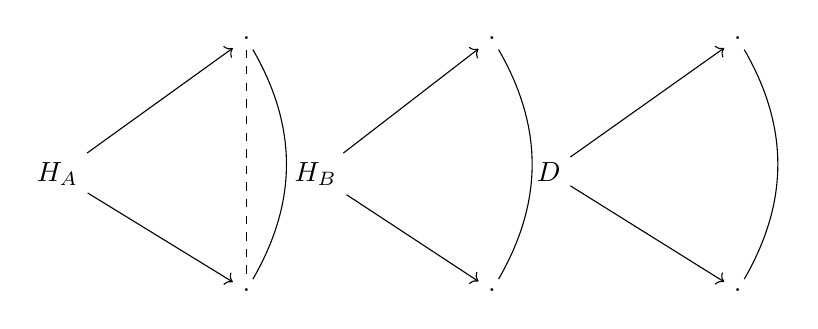
\begin{tikzpicture}[-, node distance = 3cm, scale=0.8]
        \node[anchor=north](HA){\(H_A\)};
        \node[anchor=north](HA_d1) at (3, 2){.};
        \node[anchor=north](HA_d2) at (3, -2){.};
    
        \path[->] (HA) edge node {}(HA_d1);
        \path[->] (HA) edge node {}(HA_d2);
        \path (HA_d1) edge [bend left] node {}(HA_d2);
        \path (HA_d1) [dashed] edge node {}(HA_d2);
    
        \node[anchor=north](HB) at (4.1, 0){\(H_B\)};
        \node[anchor=north](HB_d1) at (6.9, 2){.};
        \node[anchor=north](HB_d2) at (6.9, -2){.};
    
        \path[->] (HB) edge node {}(HB_d1);
        \path[->] (HB) edge node {}(HB_d2);
        \path(HB_d1) edge [bend left] node {}(HB_d2);
    
        \node[anchor=north](D) at (7.8, 0){\(D\)};
        \node[anchor=north](D_d1) at (10.8, 2){.};
        \node[anchor=north](D_d2) at (10.8, -2){.};
        
        \path[->] (D) edge node {}(D_d1);
        \path[->] (D) edge node {}(D_d2);
        \path(D_d1) edge [bend left] node {}(D_d2);
    \end{tikzpicture}
    \caption{Imperfect information Extensive Form Game between the distributor 
    and the 2 queueing systems}
    \label{fig:imperfect-info-game}
\end{figure}

The first 
queueing system \(H_A\) decides on a threshold, then the second system \(H_B\)
chooses its own threshold, without knowing the strategy of \(H_A\), and finally
the distributor makes its choice. Note here that the dotted line represents the
fact that \(H_B\) is unaware of the state of the game when making its own 
decisions. The game can thus be partitioned into a normal form game between the
two queueing systems and finding the distributor's best choice. 

In order to define the normal form game the two payoff matrices of the players 
are required. From equation \ref{eq:obj-queueing-systems} the utilities of the
players can be formulated as:

\begin{equation}
    U_{T_1, T_2}^i = \quad -\left( 
        \hat{P} - P(W_i < R) 
    \right)^2
\end{equation}

Consequently, the payoff matrices of the game can be populated by these 
utilities:

\begin{equation} \label{eq:payoff-matrices}
    A = 
    \begin{pmatrix}
        U_{1,1}^A & U_{1,2}^A & \dots & U_{1,N_B}^A \\
        U_{2,1}^A & U_{2,2}^A & \dots & U_{2,N_B}^A \\
        \vdots & \vdots & \ddots & \vdots \\
        U_{N_A,1}^A & U_{N_A,2}^A & \dots & U_{N_A,N_B}^A \\
    \end{pmatrix},
    B = 
    \begin{pmatrix}
        U_{1,1}^B & U_{1,2}^B & \dots & U_{1,N_B}^B \\
        U_{2,1}^B & U_{2,2}^B & \dots & U_{2,N_B}^B \\
        \vdots & \vdots & \ddots & \vdots \\
        U_{N_A,1}^B & U_{N_A,2}^B & \dots & U_{N_A,N_B}^B \\
    \end{pmatrix}
\end{equation}

Based on the choice of strategy of these two players the distributor will then 
make their own choice of the proportion of individuals to send to each system.

    \section{A queueing model with 2 consecutive buffer centres}

% TODO: If this is to be one paper maybe the first two paragraphs do not need to
% include so much details or even better omit some of the details in the game
% overview section.
In this section, a more in-depth explanation of the queueing model shown in 
figure \ref{fig:diagram_of_queueing_system} will be given.
This is a queuing model that consists of two waiting spaces, one for each type
of individual.

The model consists of two types of individuals; class 1 and class 2.
Class 1 individuals arrive instantly at waiting zone 1 and proceed to wait to
receive their service. 
Class 2 individuals arrive at waiting zone 2 and wait there until they are 
allowed to move to waiting zone 1. 
They are allowed to proceed only when the number of 
individuals in waiting zone 1 \textbf{and} in service is less than a 
pre-determined threshold \(T\).
When the number of individuals is equal to or exceeds this threshold, all second type individuals that arrive will remain 
\textit{``blocked''} in waiting zone 1 until the number of people in the 
system is reduced below \(T\). 
This is shown diagrammatically in figure \ref{fig:diagram_of_queueing_system}.
The parameters of the described queueing model are:

\begin{itemize}
    \item \(\lambda_i\): The arrival rate of individuals of type \(i\in\{1, 2\}\)
    \item \(\mu\): The service rate for individuals receiving service
    \item \(C\): The number of servers
    \item \(T\): The threshold at which individuals of the second type are blocked
\end{itemize}

Under the assumption that all rates (arrival and service) are Markovian the
queuing system corresponds to a Markov chain~\cite{kemeny1976markov}.
The states of the Markov chain are denoted by \((u,v)\) where:

\begin{itemize}
    \item \(u\) is the number of individuals blocked
    \item \(v\) is the number of individuals either in waiting zone 1 or in the
    service centre
\end{itemize}

We denote the state space of the Markov chain as  \(S=S(T)\) which can be 
written as the disjoint union (\ref{eq:definition_of_S_as_disjoint_union}).

\begin{align}
    S(T) =& S_1(T) \cup S_2(T) \text{ where:} \nonumber \\
    S_1(T) =& \left\{(0, v)\in\mathbb{N}_0^2 \; | \; v < T \right\} 
    \label{eq:definition_of_S_as_disjoint_union} \\
    S_2(T) =& \{(u, v)\in\mathbb{N}_0^2 \; | \; v \geq T \} \nonumber
\end{align}

The transition matrix \(Q\) of the Markov chain consists of the transition rates
between the numerous states of the model. Every entry \( Q_{ij} = 
Q_{(u_i, v_i),(u_j, v_j)} \) represents the transition rate from state 
\( i = (u_i, v_i) \) to state \( j = (u_j , v_j) \) for all 
\( (u_i, v_i), (u_j, v_j) \in S \).
The entries of \(Q\) can be calculated using the state-mapping function 
described in (\ref{eq:markov_transition_rate}): 

\begin{equation} \label{eq:markov_transition_rate}
    Q_{ij} = 
    \begin{cases}
        \Lambda, & \textbf{if } (u_i, v_i) - (u_j, v_j) = (0,-1) \textbf{ and } 
        v_i < \text{t} \\
        \lambda_1, & \textbf{if } (u_i, v_i) - (u_j, v_j) = (0,-1) 
        \textbf{ and } v_i \geq \text{t} \\
        \lambda_2, & \textbf{if } (u_i, v_i) - (u_j, v_j) = (-1,0) \\
        v_i \mu, & \textbf{if } (u_i, v_i) - (u_j, v_j) = (0,1) \textbf{ and } 
        v_i \leq C \textbf{ or} \\ & \hspace{0.37cm}(u_i, v_i) - (u_j, v_j) = 
        (1,0) \textbf{ and } v_i = T \leq C \\
        C \mu, & \textbf{if } (u_i, v_i) - (u_j, v_j) = (0,1) \textbf{ and } 
        v_i > C 
        \textbf{ or} \\ & \hspace{0.37cm}(u_i, v_i) - (u_j, v_j) = (1,0) 
        \textbf{ and } v_i = T > C\\
        -\sum_{j=1}^{|Q|}{Q_{ij}} & \textbf{if } i = j \\
        0, & \textbf{otherwise}
    \end{cases}
\end{equation}

Note that \(\Lambda\) here denotes the overall arrival rate in the model by both 
classes of individuals (i.e. \(\Lambda = \lambda_1 + \lambda_2\)). 
A visualisation of how the transition rates relate to the states of the model 
can be seen in the general Markov chain model shown in figure 
\ref{fig:general-markov-model}.

\documentclass{article}

\usepackage{amsmath}
\usepackage{amsfonts} 
\usepackage{geometry}
\usepackage{multicol}
\usepackage{float}
% \usepackage{mathtools}
% \usepackage{graphicx}
% \usepackage{soul}
% \usepackage{indentfirst}
\usepackage{tikz}
\usetikzlibrary{calc, automata, chains, arrows.meta, math}
\setcounter{MaxMatrixCols}{20}


\title{A game theoretic model of the behavioural gaming that takes place at the EMS - ED interface}

\author{
    Michalis Panayides, 
    Paul Harper, 
    Vince Knight
}

\begin{document}

\maketitle

\documentclass{article}

\usepackage{amsmath}
\usepackage{amsfonts} 
\usepackage{geometry}
\usepackage{multicol}
\usepackage{float}
% \usepackage{mathtools}
% \usepackage{graphicx}
% \usepackage{soul}
% \usepackage{indentfirst}
\usepackage{tikz}
\usetikzlibrary{calc, automata, chains, arrows.meta, math}
\setcounter{MaxMatrixCols}{20}


\title{A game theoretic model of the behavioural gaming that takes place at the EMS - ED interface}

\author{
    Michalis Panayides, 
    Paul Harper, 
    Vince Knight
}

\begin{document}

\maketitle

\input{Abstract/main.tex}


\newpage
\tableofcontents

\newpage
\input{Introduction/main.tex}

\newpage
\input{Game_theory_component/main.tex}

\newpage
\input{MarkovChain/markov_chain_model/main.tex}
\input{MarkovChain/expressions_from_pi/main.tex}
\input{MarkovChain/markov_example/main.tex}

\newpage
\input{BehaviouralMethodology/main.tex}

\newpage
\input{Application_EMS_ED/main.tex}

\newpage
\input{Conclusion/main.tex}


\end{document}


\newpage
\tableofcontents

\newpage
\documentclass{article}

\usepackage{amsmath}
\usepackage{amsfonts} 
\usepackage{geometry}
\usepackage{multicol}
\usepackage{float}
% \usepackage{mathtools}
% \usepackage{graphicx}
% \usepackage{soul}
% \usepackage{indentfirst}
\usepackage{tikz}
\usetikzlibrary{calc, automata, chains, arrows.meta, math}
\setcounter{MaxMatrixCols}{20}


\title{A game theoretic model of the behavioural gaming that takes place at the EMS - ED interface}

\author{
    Michalis Panayides, 
    Paul Harper, 
    Vince Knight
}

\begin{document}

\maketitle

\input{Abstract/main.tex}


\newpage
\tableofcontents

\newpage
\input{Introduction/main.tex}

\newpage
\input{Game_theory_component/main.tex}

\newpage
\input{MarkovChain/markov_chain_model/main.tex}
\input{MarkovChain/expressions_from_pi/main.tex}
\input{MarkovChain/markov_example/main.tex}

\newpage
\input{BehaviouralMethodology/main.tex}

\newpage
\input{Application_EMS_ED/main.tex}

\newpage
\input{Conclusion/main.tex}


\end{document}

\newpage
\documentclass{article}

\usepackage{amsmath}
\usepackage{amsfonts} 
\usepackage{geometry}
\usepackage{multicol}
\usepackage{float}
% \usepackage{mathtools}
% \usepackage{graphicx}
% \usepackage{soul}
% \usepackage{indentfirst}
\usepackage{tikz}
\usetikzlibrary{calc, automata, chains, arrows.meta, math}
\setcounter{MaxMatrixCols}{20}


\title{A game theoretic model of the behavioural gaming that takes place at the EMS - ED interface}

\author{
    Michalis Panayides, 
    Paul Harper, 
    Vince Knight
}

\begin{document}

\maketitle

\input{Abstract/main.tex}


\newpage
\tableofcontents

\newpage
\input{Introduction/main.tex}

\newpage
\input{Game_theory_component/main.tex}

\newpage
\input{MarkovChain/markov_chain_model/main.tex}
\input{MarkovChain/expressions_from_pi/main.tex}
\input{MarkovChain/markov_example/main.tex}

\newpage
\input{BehaviouralMethodology/main.tex}

\newpage
\input{Application_EMS_ED/main.tex}

\newpage
\input{Conclusion/main.tex}


\end{document}

\newpage
\documentclass{article}

\usepackage{amsmath}
\usepackage{amsfonts} 
\usepackage{geometry}
\usepackage{multicol}
\usepackage{float}
% \usepackage{mathtools}
% \usepackage{graphicx}
% \usepackage{soul}
% \usepackage{indentfirst}
\usepackage{tikz}
\usetikzlibrary{calc, automata, chains, arrows.meta, math}
\setcounter{MaxMatrixCols}{20}


\title{A game theoretic model of the behavioural gaming that takes place at the EMS - ED interface}

\author{
    Michalis Panayides, 
    Paul Harper, 
    Vince Knight
}

\begin{document}

\maketitle

\input{Abstract/main.tex}


\newpage
\tableofcontents

\newpage
\input{Introduction/main.tex}

\newpage
\input{Game_theory_component/main.tex}

\newpage
\input{MarkovChain/markov_chain_model/main.tex}
\input{MarkovChain/expressions_from_pi/main.tex}
\input{MarkovChain/markov_example/main.tex}

\newpage
\input{BehaviouralMethodology/main.tex}

\newpage
\input{Application_EMS_ED/main.tex}

\newpage
\input{Conclusion/main.tex}


\end{document}
\subsection{Performance Measures}
One may easily derive the average number of individuals that are at any given state 
using \( pi \). 
The average number of individuals in state \( i \) can be calculated by multiplying 
the number of individuals that are present in state \( i \) with the probability 
of being at that particular state (i.e \(\pi_i (u_i + v_i)\)). 
Using this logic it is possible to calculate any performance measures that are related 
to the mean number of individuals in the system.


Average number of people in the system: 
\begin{equation}
    L = \sum_{i=1}^{|\pi|} \pi_i (u_i + v_i)
\end{equation} 

Average number of people in the service centre: 
\begin{equation}
    L_H = \sum_{i=1}^{|\pi|} \pi_i v_i
\end{equation}

Average number of people in the buffer centre:
\begin{equation}
    L_A = \sum_{i=1}^{|\pi|} \pi_i u_i
\end{equation}

Consequently getting the performance measures that are related to the duration of 
time is not as straightforward. 
Such performance measures are the mean waiting time in the system and the mean time 
blocked in the system. 
Under the scope of this study three approaches have been considered to calculate these 
performance measures; a direct approach, a recursive algorithm and consequently a
closed-form formula.

The research question that needs to be answered here is: ``When a class 1/2 
individuals enters the system, what is the expected time that they will have to 
wait?''. 
In order to formulate the answer to that question one needs to consider all possible 
scenarios of what state the system can be in when an individual arrives. 
Furthermore, different formulas arises for class 1 individuals 
and a different one for class 2 individuals.

\subsubsection{Mean waiting time} 
Upon closer inspection of the recursive formula a more compact formula can arise. 
The equivalent closed-form formula eliminates the need for recursion and thus makes 
the computation of waiting times much more efficient. 
Just like in the recursive part there are two formulas; one for \textit{class 1} 
and one for class 2 individuals. 
The formulas are given by:

\begin{equation} \label{eq:closed_form_waiting_others}
    W^{(1)} = \frac{\sum_{\substack{(u,v) \, \in S_A^{(1)} \\ v \geq C}} 
    \frac{1}{C \mu} \times (v-C+1) \times \pi(u,v)}{\sum_{(u,v) \, 
    \in S_A^{(1)}} \pi(u,v)}
\end{equation}
    
\begin{equation}\label{eq:closed_form_waiting_ambulance}
    W^{(2)} = \frac{\sum_{\substack{(u,v) \, \in S_A^{(2)} \\ min(v,T) \geq C}} 
    \frac{1}{C \mu} \times (\min(v+1,T)-C) \times \pi(u,v)}{\sum_{(u,v) \, 
    \in S_A^{(2)}} \pi(u,v)}
\end{equation}

Note here that the summation, in both equations \ref{eq:closed_form_waiting_others} 
and \ref{eq:closed_form_waiting_ambulance}, goes through all states in the set of 
accepting 
states of either class 1 or class 2 individuals respectively, where a wait 
incurs. 
In equation \ref{eq:closed_form_waiting_others} that includes all states \((u,v)\) 
in the set of accepting states of class 1 individuals such that \( v \geq C\); i.e. 
whenever an arrival occurs and the system is at a state where the number of individuals 
in the system is more than or equal to $C$. 
Consequently, for the states that are included in the summation the expression 
\( v-C+1 \) indicates the amount of people in service one would have to wait for 
upon arrival at the hospital.

Additionally, the minimisation function in equation 
\ref{eq:closed_form_waiting_ambulance} 
ensures that when a class 2 individual arrives at any state 
that is greater than the predetermined threshold, the wait that the individual will 
have to endure remains the same. 
In essence, the expression \(\min(v+1,T) - C\) returns the number of people in line 
in front of a particular individual upon arrival.


\subsubsection{Overall Waiting Time}

Consequently, the overall waiting time should can be estimated by a linear combination 
of the waiting times of class 1 and class 2 individuals. 
The overall waiting time can be then given by the following equation where \(c_1\) 
and \(c_2\) are the coefficients of each individual's type waiting time:

\begin{equation}\label{overall_waiting_time_coeff}
    W = c_1 W^{(1)} + c_2 W^{(2)}
\end{equation}

The two coefficients represent the proportion of individuals of each type that 
traversed through the model. 
Theoretically, getting these percentages should be as simple as looking at the arrival 
rates of each type but in practise if the service centre or the buffer centre 
is full, some individuals may be lost to the system. 
Thus, one should account for the probability that an individual is lost to the system. 
This probability can be easily calculated by using the two sets of accepting states 
\(S_A^{(2)}\) and \(S_A^{(1)}\) defined earlier in equations.
Let us define here the probability, for either class type, that an individual 
is not lost in the system by:

\begin{equation*}
    P(L'_1) = \sum_{(u,v) \, \in S_A^{(1)}} \pi(u,v) \hspace{2cm}
    P(L'_2) = \sum_{(u,v) \, \in S_A^{(2)}} \pi(u,v)
\end{equation*}

Having defined these probabilities one may combine them with the arrival rates of 
each class type in such a way to get the expected proportions of class 1 and 
class 2 individuals in the model. 
Thus, by using these values as the coefficient of equation 
\ref{overall_waiting_time_coeff} 
the resultant equation can be used to get the overall waiting time. 
Note here that the equation below gets the overall waiting time for both the recursive 
and the closed-form formula.

\begin{equation}\label{overall_waiting_time}
    W = \frac{\lambda_1 P(L'_1)}{\lambda_2 P(L'_2) + \lambda_1 P(L'_1)} W^{(1)} + 
    \frac{\lambda_2 P(L'_2)}{\lambda_2 P(L'_2) + \lambda_1 P(L'_1)} W^{(2)}
\end{equation}



\subsubsection{Mean blocking time}
Unlike the waiting time, the blocking time is only calculated for class 2 individuals.  
That is because class 1 individuals cannot be blocked. 
Thus, one only needs to consider the pathway of class 2 individuals to get the 
mean blocking time of the system. 
Blocking occurs at states \((u,v)\) where \(u > 0 \). 
Thus, the set of blocking states can be defined as:

\begin{equation*}
    S_b = \{(u,v) \in S \; | \; u > 0\}
\end{equation*}
 
In order to not consider individuals that will be lost to the system, the set of 
accepting states needs to be taken into account. The set of accepting states is given by:

\begin{equation*}
    S_A^{(2)}=
    \begin{cases}
        \{(u, v) \in S \; | \; u < M \} & \textbf{if } T \leq N\\
        \{(u, v) \in S \; | \; v < N \} & \textbf{otherwise}
    \end{cases}
\end{equation*}

For the waiting time formula,
the mean sojourn time for each state was considered,
ignoring any arrivals. Here, the same approach is used but ignoring only class 2
arrivals. That is because for the waiting time formula, once an individual enters 
the service centre (i.e. starts waiting) any individual arriving after them will 
not affect their
pathway. That is not the case for blocking time. When a class 2 individual is 
blocked, 
any class 1 individual that arrives will cause the blocked individual to remain 
blocked for more time. Therefore, class 1 arrivals are considered here:

\begin{equation}\label{eq:time_in_state_blocking_time}
    c(u,v) = 
    \begin{cases}
        \frac{1}{\min(v,C) \mu}, & \text{if } v = C\\
        \frac{1}{\min(v,C) \mu + \lambda_1}, & \text{otherwise}
    \end{cases}
\end{equation}
 
In equation \ref{eq:time_in_state_blocking_time}, both service completions and 
class 1 arrivals are considered. 
Thus, from a blocked individual's perspective whenever the system moves from one 
state \((u,v)\)
to another state it can either:

\begin{itemize}
    \item be because of a service being completed: we will denote the probability 
    of this happening by \(p_s(u,v)\). 
    \item be because of an arrival of an individual of class 1: denoting such 
    probability by \(p_o(u,v)\).
\end{itemize}
The probabilities are given by:

\begin{equation*}
    p_s(u,v) = \frac{\min(v,C)\mu}{\lambda_1 + \min(v,C)\mu}, \qquad
    p_o(u,v) = \frac{\lambda_1}{\lambda_1 + \min(v,C)\mu}
\end{equation*}


Having defined \(c(u,v)\) and \(S_b\) a formula for the blocking time that is
expected to occur at each state can be given by:

\begin{equation}\label{eq:blocking-time-at-each-state}
    b(u,v) = 
    \begin{cases} 
        0, & \textbf{if } (u,v) \notin S_b \\
        c(u,v) + b(u - 1, v), & \textbf{if } v = N = T\\
        c(u,v) + b(u, v-1), & \textbf{if } v = N \neq T \\
        c(u,v) + p_s(u,v) b(u-1, v) + p_o(u,v) b(u, v+1), & \textbf{if } u > 0 
        \textbf{ and } v = T \\
        c(u,v) + p_s(u,v) b(u, v-1) + p_o(u,v) b(u, v+1), & \textbf{otherwise} \\
    \end{cases}
\end{equation}

Equation 
(\ref{eq:blocking-time-at-each-state}) will not be solved recursively. 
A direct approach will be used to solve this equation here. 
By enumerating all equations of (\ref{eq:blocking-time-at-each-state}) for all 
states \((u,v)\) that belong in \(S_b\) 
a system of linear equations arises where the unknown variables are all the \(b(u,v)\)
terms.
For instance, let us consider a Markov model where \(C=2, T=3, N=6, M=2\). 
The Markov model is shown in Figure \ref{fig:example-algeb-blocking}
and the equivalent equations are 
(\ref{eq:first_eq_of_blocking_example})-(\ref{eq:last_eq_of_blocking_example}).
The equations considered here are only the ones that correspond to the blocking 
states.

\begin{multicols*}{2}
    \begin{figure}[H]
        \scalebox{0.50}{\input{MarkovChain/expressions_from_pi/example_model_2362/main.tex}}
        \caption{Example of Markov chain}
        \label{fig:example-algeb-blocking}
    \end{figure}
    \columnbreak
    \begin{align}
        b(1,2) &= c(1,2) + p_o b(1,3) \label{eq:first_eq_of_blocking_example} \\
        b(1,3) &= c(1,3) + p_s b(1,2) + p_o b(1,4) \\
        b(1,4) &= c(1,4) + b(1,3) \\
        b(2,2) &= c(2,2) + p_s b(1,2) + p_o b(2,3) \\
        b(2,3) &= c(2,3) + p_s b(2,2) + p_o b(1,4) \\
        b(2,4) &= c(2,4) + b(2,3)\label{eq:last_eq_of_blocking_example}
    \end{align}
\end{multicols*}

Additionally, the above equations can be transformed into a linear system of the 
form \(Zx=y\) where:

\begin{equation}\label{eq:example-algebaric-approach-blocking-time}
    Z=
    \begin{pmatrix}
        -1 & p_o & 0 & 0 & 0 & 0 \\ %(1,2)
        p_s & -1 & p_o & 0 & 0 & 0 \\ %(1,3)
        0 & 1 & -1 & 0 & 0 & 0 \\ %(1,4)
        p_s & 0 & 0 & -1 & p_o & 0\\ %(2,2)
        0 & 0 & 0 & p_s & -1 & p_o \\ %(2,3)
        0 & 0 & 0 & 0 & 1 & -1 \\ %(2,4)
    \end{pmatrix},
    x=
    \begin{pmatrix}
        b(1,2) \\
        b(1,3) \\
        b(1,4) \\
        b(2,2) \\
        b(2,3) \\
        b(2,4) \\
    \end{pmatrix}, 
    y=
    \begin{pmatrix}
        -c(1,2) \\
        -c(1,3) \\
        -c(1,4) \\
        -c(2,2) \\
        -c(2,3) \\
        -c(2,4) \\
    \end{pmatrix}
\end{equation}

A more generalised form of the equations in 
(\ref{eq:example-algebaric-approach-blocking-time})
can thus be given for any value of \(C,T,N,M\) by:

\begin{align}
    b(1,T) =& c(1, T) + p_o b(1, T + 1) \label{eq:first_eq_of_blocking_general}\\
    b(1,T + 1) =& c(1, T + 1) + p_s(1, T) + p_o b(1, T + 1) \\
    b(1,T + 2) =& c(1, T + 2) + p_s(1, T + 1) + p_o b(1, T + 3) \\
    & \vdots \nonumber \\
    b(1, N) =& c(1, N) + b(1, N - 1) \\
    b(2, T) =& c(2, T) + p_s b(1, T) + p_o b(2, T + 1) \\
    b(2, T + 1) =& c(2, T + 1) + p_s b(2, T) + p_o b(2, T + 2) \\
    & \vdots \nonumber \\
    b(M, T) =& c(M, T) + b(M, T-1) \label{eq:last_eq_of_blocking_general}
\end{align}

The equivalent matrix form of the linear system of equations 
(\ref{eq:first_eq_of_blocking_general}) - (\ref{eq:last_eq_of_blocking_general})
is given by \(Zx=y\), where:
\begin{equation}\label{eq:general-algebaric-approach-blocking-time}
    \scalebox{0.9}{
        \(
        Z = 
        \begin{pmatrix}
            -1 & p_o & 0 & \dots & 0 & 0 & 0 & 0 & 0 & \dots & 0 & 0 \\ %(1,T)
            p_s & -1 & p_o & \dots & 0 & 0 & 0 & 0 & 0 & \dots & 0 & 0 \\ %(1,T+1)
            0 & p_s & -1 & \dots & 0 & 0 & 0 & 0 & 0 & \dots & 0 & 0 \\ %(1,T+2)
            \vdots & \vdots & \vdots & \ddots & \vdots & \vdots & \vdots & \vdots & 
            \vdots & \ddots & \vdots & \vdots \\ 
            0 & 0 & 0 & \dots & 1 & -1 & 0 & 0 & 0 & \dots & 0 & 0 \\ %(1,N)
            p_s & 0 & 0 & \dots & 0 & 0 & -1 & p_o & 0 & \dots & 0 & 0 \\ %(2,T)
            0 & 0 & 0 & \dots & 0 & 0 & p_s & -1 & p_o & \dots & 0 & 0 \\ %(2,T+1)
            \vdots & \vdots & \vdots & \ddots & \vdots & \vdots & \vdots & \vdots & 
            \vdots & \ddots & \vdots & \vdots \\ 
            0 & 0 & 0 & \dots & 0 & 0 & 0 & 0 & 0 & \dots & 1 & -1 \\ %(M,T)
        \end{pmatrix},
        x = 
        \begin{pmatrix}
            b(1,T) \\
            b(1,T+1) \\
            b(1,T+2) \\
            \vdots \\
            b(1,N) \\
            b(2,T) \\
            b(2,T+1) \\
            \vdots \\
            b(M,T) \\
        \end{pmatrix}, 
        y= 
        \begin{pmatrix}
            -c(1,T) \\
            -c(1,T+1) \\
            -c(1,T+2) \\
            \vdots \\
            -c(1,N) \\
            -c(2,T) \\
            -c(2,T+1) \\
            \vdots \\
            -c(M,T) \\
        \end{pmatrix}
        \)
    }
\end{equation}

Thus, having calculated the mean blocking time for all blocking states \(b(u,v)\), 
it only remains to put them together in a formula.
The resultant blocking time formula is given by:

\begin{equation}\label{eq:algebraic-blocking-time}
    B = \frac{\sum_{(u,v) \in S_A} \pi_{(u,v)} \; b(u,v)}{\sum_{(u,v) \in S_A} 
    \pi_{(u,v)}}
\end{equation}

\documentclass{article}

\usepackage{amsmath}
\usepackage{amsfonts} 
\usepackage{geometry}
\usepackage{multicol}
\usepackage{float}
% \usepackage{mathtools}
% \usepackage{graphicx}
% \usepackage{soul}
% \usepackage{indentfirst}
\usepackage{tikz}
\usetikzlibrary{calc, automata, chains, arrows.meta, math}
\setcounter{MaxMatrixCols}{20}


\title{A game theoretic model of the behavioural gaming that takes place at the EMS - ED interface}

\author{
    Michalis Panayides, 
    Paul Harper, 
    Vince Knight
}

\begin{document}

\maketitle

\input{Abstract/main.tex}


\newpage
\tableofcontents

\newpage
\input{Introduction/main.tex}

\newpage
\input{Game_theory_component/main.tex}

\newpage
\input{MarkovChain/markov_chain_model/main.tex}
\input{MarkovChain/expressions_from_pi/main.tex}
\input{MarkovChain/markov_example/main.tex}

\newpage
\input{BehaviouralMethodology/main.tex}

\newpage
\input{Application_EMS_ED/main.tex}

\newpage
\input{Conclusion/main.tex}


\end{document}

\newpage
\documentclass{article}

\usepackage{amsmath}
\usepackage{amsfonts} 
\usepackage{geometry}
\usepackage{multicol}
\usepackage{float}
% \usepackage{mathtools}
% \usepackage{graphicx}
% \usepackage{soul}
% \usepackage{indentfirst}
\usepackage{tikz}
\usetikzlibrary{calc, automata, chains, arrows.meta, math}
\setcounter{MaxMatrixCols}{20}


\title{A game theoretic model of the behavioural gaming that takes place at the EMS - ED interface}

\author{
    Michalis Panayides, 
    Paul Harper, 
    Vince Knight
}

\begin{document}

\maketitle

\input{Abstract/main.tex}


\newpage
\tableofcontents

\newpage
\input{Introduction/main.tex}

\newpage
\input{Game_theory_component/main.tex}

\newpage
\input{MarkovChain/markov_chain_model/main.tex}
\input{MarkovChain/expressions_from_pi/main.tex}
\input{MarkovChain/markov_example/main.tex}

\newpage
\input{BehaviouralMethodology/main.tex}

\newpage
\input{Application_EMS_ED/main.tex}

\newpage
\input{Conclusion/main.tex}


\end{document}

\newpage
\section{EMS-ED application}

\subsection{Application}

\subsection{Data analysis of generated problem}

\newpage
\documentclass{article}

\usepackage{amsmath}
\usepackage{amsfonts} 
\usepackage{geometry}
\usepackage{multicol}
\usepackage{float}
% \usepackage{mathtools}
% \usepackage{graphicx}
% \usepackage{soul}
% \usepackage{indentfirst}
\usepackage{tikz}
\usetikzlibrary{calc, automata, chains, arrows.meta, math}
\setcounter{MaxMatrixCols}{20}


\title{A game theoretic model of the behavioural gaming that takes place at the EMS - ED interface}

\author{
    Michalis Panayides, 
    Paul Harper, 
    Vince Knight
}

\begin{document}

\maketitle

\input{Abstract/main.tex}


\newpage
\tableofcontents

\newpage
\input{Introduction/main.tex}

\newpage
\input{Game_theory_component/main.tex}

\newpage
\input{MarkovChain/markov_chain_model/main.tex}
\input{MarkovChain/expressions_from_pi/main.tex}
\input{MarkovChain/markov_example/main.tex}

\newpage
\input{BehaviouralMethodology/main.tex}

\newpage
\input{Application_EMS_ED/main.tex}

\newpage
\input{Conclusion/main.tex}


\end{document}


\end{document}


In order to consider this model numerically an adjustment needs to be made. 
The problem defined above assumes no upper boundary to the number of individuals 
that can wait for service or for the ones that are blocked in the buffer centre. 
Therefore, a different state space \( \tilde S \) is constructed where 
\( \tilde S \subseteq S \) and there is a maximum allowed number of individuals 
\(N\) that can be in the system and a maximum allowed number of individuals 
\(M\) that can be blocked in the buffer centre:

\begin{equation}
    \tilde S = \left\{ (u, v) \in S\;| u \leq M, v\leq N \right\}
\end{equation}


\subsection{Performance Measures}


The transition matrix \( Q \) defined in \ref{eq:markov_transition_rate} can be 
used to get the probability vector \( \pi \).
The vector \( \pi \) is commonly used to study stochastic systems and it's main
purpose is to keep track of the probability of being at any given state of 
the system.
The term \textit{steady state} refers to the instance of the vector \( \pi \) 
where the probabilities of being at any state become stable over time. 
Thus, by considering the steady state vector \( \pi \) the relationship between 
it and \( Q \) is given by:

\[
    \frac{d\pi}{dt} = \pi Q = 0
\]

Using vector \(\pi\) there are numerous performance measures of the model that 
can be calculated. 
The following equations utilise \(\pi\) to get performance measures on the 
average number of people at certain sets of state.

\begin{itemize}
    \item Average number of people in the system: 
        \[L = \sum_{i=1}^{|\pi|} \pi_i (u_i + v_i)\]
    \item Average number of people in the service centre: 
        \[L_H = \sum_{i=1}^{|\pi|} \pi_i v_i\]
    \item Average number of people in waiting zone 2:
        \[L_A = \sum_{i=1}^{|\pi|} \pi_i u_i\] 
\end{itemize}

Consequently, there are some additional performance measures of interest that
are not as straightforward to calculate.
Such performance measures are the mean waiting time in the system (for both 
class 1 and class 2 individuals), the mean time blocked in waiting zone 2 (only 
valid for class 2 individuals) and the proportion of individuals that wait in 
waiting zone 1 within a predefined time target.

\subsubsection{Waiting time} \label{sec:waiting_time}

Waiting time is the amount of time that individuals from either class wait in 
waiting zone 1 so that they can receive their service. 
For a given set of parameters there are three different performance measures 
around the mean waiting time that can be calculated; the mean waiting time of
class 1 individuals, the mean waiting time of class 2 individuals and the 
overall mean waiting time. 

Since some of the individuals can be lost to the model, a new set of states 
needs to be defined; the set of \textit{accepting states}. 
That is the set of states that the model is able to accept a certain type of
individual. 
The set of accepting states for class 1 individuals is defined as:

\begin{equation}\label{eq:accepting_states_class_1}
    S_A^{(1)} = \{(u, v) \in S \; | \; v < N \}
\end{equation}

In essence, for class 1 individuals, this is the set of states that are not on 
the last column of states in the Markov chain.
Equivalently, the set of accepting states for class 2 individuals is defined as:

\begin{equation}\label{eq:accepting_states_class_2}
    S_A^{(2)}=
    \begin{cases}
        \{(u, v) \in S \; | \; u < M \}, & \textbf{if } T \leq N\\
        \{(u, v) \in S \; | \; v < N \}, & \textbf{otherwise}
    \end{cases}
\end{equation}

Note here that if the threshold is less than or equal the total capacity of the
system the set includes all states that are not on the last column of the 
Markov chain.
Otherwise, the set of accepting state is identical to 
\ref{eq:accepting_states_class_1}. Thus, the expressions for the waiting times 
for class 1 and class 2 individuals are given by:

\begin{equation} \label{eq:closed_form_waiting_class_1}
    W^{(1)} = \frac{\sum_{\substack{(u,v) \, \in S_A^{(1)} \\ v \geq C}} 
    \frac{1}{C \mu} \times (v-C+1) \times \pi(u,v)}{\sum_{(u,v) \, 
    \in S_A^{(1)}} \pi(u,v)}
\end{equation}
    
\begin{equation}\label{eq:closed_form_waiting_class_2}
    W^{(2)} = \frac{\sum_{\substack{(u,v) \, \in S_A^{(2)} \\ min(v,T) \geq C}} 
    \frac{1}{C \mu} \times (\min(v+1,T)-C) \times \pi(u,v)}{\sum_{(u,v) \, 
    \in S_A^{(2)}} \pi(u,v)}
\end{equation}

Consequently, the overall waiting time can be estimated by a linear combination 
of \(W_1\) and \(W_2\). 
Thus, the overall waiting time can calculated by the following equation where 
\(c_1\) and \(c_2\) are the coefficients of the terms:

\begin{equation}\label{eq:overall_waiting_time_coeff}
    W = c_1 W^{(1)} + c_2 W^{(2)}
\end{equation}

The two coefficients represent the proportion of individuals of each type that 
did not get lost and traversed through the model.
Thus, one should account for the probability that an individual is lost to the 
system. 
This probability can be easily calculated by using the two sets of accepting 
states \(S_A^{(2)}\) and \(S_A^{(1)}\) defined in equations 
\ref{eq:accepting_states_class_1} and \ref{eq:accepting_states_class_2}. 
Using these equations the probability, for either class type, that an individual 
is not lost in the system is given by:

\begin{equation*}
    P(L'_1) = \sum_{(u,v) \, \in S_A^{(1)}} \pi(u,v) \hspace{2cm}
    P(L'_2) = \sum_{(u,v) \, \in S_A^{(2)}} \pi(u,v)
\end{equation*}
 
Thus, by using these values as the coefficient of equation 
\ref{eq:overall_waiting_time_coeff} the resultant equation can be used to get 
the overall waiting time. 

\begin{equation}\label{eq:overall_waiting_time}
    W = \frac{\lambda_1 P(L'_1)}{\lambda_2 P(L'_2) + \lambda_1 P(L'_1)} W^{(1)} + 
    \frac{\lambda_2 P(L'_2)}{\lambda_2 P(L'_2) + \lambda_1 P(L'_1)} W^{(2)}
\end{equation}


\subsubsection{Blocking time}

% TODO: Possibly replace the contents of this section with the ones for the 
% closed form formula of the blocking time
% Currently the direct approach one is shown

Unlike the waiting time, the blocking time is only calculated for individuals of
the second type.  
That is because individuals of the first type cannot be blocked. 
Thus, one only needs to consider the pathway of type 2 individuals to get the 
mean blocking time of the system. 
The set of states where individuals can be blocked is defined as:

\begin{equation} \label{eq:set_of_blocking_states}
    S_b = \{(u,v) \in S \; | \; u > 0\}
\end{equation}
 
In order to not consider individuals that will be lost to the system, the set of 
accepting states needs to be taken into consideration. 
As defined in section \ref{sec:waiting_time}, the set of accepting states is 
given by (\ref{eq:accepting_states_type_2}):

\begin{equation*}
    S_A^{(2)}=
    \begin{cases}
        \{(u, v) \in S \; | \; u < M \} & \textbf{if } T \leq N\\
        \{(u, v) \in S \; | \; v < N \} & \textbf{otherwise}
    \end{cases}
\end{equation*}

The mean sojourn time for each state is given by the inverse of the out-flow of
that state.
However, whenever a type 2 individual arrives at the system, no subsequent 
arrival of another type 2 individual can affect its pathway or total time in 
the system.
Therefore, looking at the mean time in the system from the perspective of an 
individual of the second type, all such type 2 arrivals need to be ignored.
Note here that this is not the case for individuals of the first type.
Whenever a type 2 individual is blocked and a type 1 individual arrives the type
2 individuals will remain blocked for some additional amount of time.
Thus, the mean time that a type 2 individual spends at each state is given by:

\begin{equation}\label{eq:time_in_state_blocking_time}
    c(u,v) = 
    \begin{cases}
        \frac{1}{\min(v,C) \mu}, & \text{if } v = N\\
        \frac{1}{\lambda_1 + \min(v,C) \mu}, & \text{otherwise}
    \end{cases}
\end{equation}
 
In equation (\ref{eq:time_in_state_blocking_time}), both service completions and 
type 1 arrivals are considered. 
Thus, from a blocked individual's perspective whenever the system moves from one 
state \((u,v)\)
to another state it can either:

\begin{itemize}
    \item be because of a service being completed: we will denote the probability 
    of this happening by \(p_s(u,v)\). 
    \item be because of an arrival of an individual of type 1: denoting such 
    probability by \(p_o(u,v)\).
\end{itemize}
The probabilities are given by:

\begin{equation*}
    p_s(u,v) = \frac{\min(v,C)\mu}{\lambda_1 + \min(v,C)\mu}, \qquad
    p_o(u,v) = \frac{\lambda_1}{\lambda_1 + \min(v,C)\mu}
\end{equation*}


Having defined \(c(u,v)\) and \(S_b\) a formula for the blocking time that is
expected to occur at each state can be given by:

\begin{equation}\label{eq:general_blocking_time_at_each_state}
    b(u,v) = 
    \begin{cases} 
        0, & \textbf{if } (u,v) \notin S_b \\
        c(u,v) + b(u - 1, v), & \textbf{if } v = N = T\\
        c(u,v) + b(u, v-1), & \textbf{if } v = N \neq T \\
        c(u,v) + p_s(u,v) b(u-1, v) + p_o(u,v) b(u, v+1), & \textbf{if } u > 0 
        \textbf{ and } \vspace{-0.2cm} \\ 
        & \quad v = T \\
        c(u,v) + p_s(u,v) b(u, v-1) + p_o(u,v) b(u, v+1), & \textbf{otherwise} \\
    \end{cases}
\end{equation}

A direct approach will be used to solve this equation here. 
By enumerating all equations of ((\ref{eq:general_blocking_time_at_each_state})) 
for all states \((u,v)\) that belong in \(S_b\) 
a system of linear equations arises where the unknown variables are all the 
\(b(u,v)\) terms. 
Note here that these equations correspond to all blocking states as defined in
(\ref{eq:set_of_blocking_states}). 
Equations that correspond to non-blocking states have a value of \(0\) as 
defined in (\ref{eq:general_blocking_time_at_each_state})
The general form of the equation in terms of \(C,T,N \text{ and } M\) is given by: 

\begin{align}
    b(1,T) \quad &= \quad c(1, T) + p_o b(1, T + 1) \label{eq:first_eq_of_blocking_general}\\
    b(1,T + 1) \quad &= \quad c(1, T + 1) + p_s b(1, T) + p_o b(1, T + 1) \\
    b(1,T + 2) \quad &= \quad c(1, T + 2) + p_s b(1, T + 1) + p_o b(1, T + 3) \\
    & \ \, \vdots \nonumber \\
    b(1, N) \quad &= \quad c(1, N) + b(1, N - 1) \\
    b(2, T) \quad &= \quad c(2, T) + p_s b(1, T) + p_o b(2, T + 1) \\
    b(2, T + 1) \quad &= \quad c(2, T + 1) + p_s b(2, T) + p_o b(2, T + 2) \\
    & \ \, \vdots \nonumber \\
    b(M - 1, N) \quad &= \quad c(M, N - 1) + b(M, N-1) \\ 
    b(M, T) \quad &= \quad c(T, N) + p_s b(T-1, N) + p_o b(T, N+1) \\
    & \ \, \vdots \nonumber \\
    b(M, N) \quad &= \quad c(M, N) + b(M, N-1) \label{eq:last_eq_of_blocking_general}
\end{align}

The equivalent matrix notation of the linear system of equations 
((\ref{eq:first_eq_of_blocking_general})) - ((\ref{eq:last_eq_of_blocking_general}))
is given by \(Zx=y\), where:
\begin{equation}\label{eq:general_algebaric_approach_blocking_time}
    \scalebox{0.73}{\(
        Z = 
        \begin{pmatrix}
            -1 & p_o & 0 & \dots & 0 & 0 & 0 & 0 & 0 & \dots & 0 & 0 \\ %(1,T)
            p_s & -1 & p_o & \dots & 0 & 0 & 0 & 0 & 0 & \dots & 0 & 0 \\ %(1,T+1)
            0 & p_s & -1 & \dots & 0 & 0 & 0 & 0 & 0 & \dots & 0 & 0 \\ %(1,T+2)
            \vdots & \vdots & \vdots & \ddots & \vdots & \vdots & \vdots & 
            \vdots & \vdots & \ddots & \vdots & \vdots \\ 
            0 & 0 & 0 & \dots & 1 & -1 & 0 & 0 & 0 & \dots & 0 & 0 \\ %(1,N)
            p_s & 0 & 0 & \dots & 0 & 0 & -1 & p_o & 0 & \dots & 0 & 0 \\ %(2,T)
            0 & 0 & 0 & \dots & 0 & 0 & p_s & -1 & p_o & \dots & 0 & 0 \\ %(2,T+1)
            \vdots & \vdots & \vdots & \ddots & \vdots & \vdots & \vdots & 
            \vdots & \vdots & \ddots & \vdots & \vdots \\ 
            0 & 0 & 0 & \dots & 0 & 0 & 0 & 0 & 0 & \dots & 1 & -1 \\ %(M,N)
        \end{pmatrix},
        x = 
        \begin{pmatrix}
            b(1,T) \\
            b(1,T+1) \\
            b(1,T+2) \\
            \vdots \\
            b(1,N) \\
            b(2,T) \\
            b(2,T+1) \\
            \vdots \\
            b(M,N) \\
        \end{pmatrix}, 
        y= 
        \begin{pmatrix}
            -c(1,T) \\
            -c(1,T+1) \\
            -c(1,T+2) \\
            \vdots \\
            -c(1,N) \\
            -c(2,T) \\
            -c(2,T+1) \\
            \vdots \\
            -c(M,N) \\
        \end{pmatrix}
    \)}
\end{equation}

Thus, having calculated the mean blocking time for all blocking states \(b(u,v)\), 
it only remains to put them together in a formula.
The resultant formula for the mean blocking time is given by:

\begin{equation}\label{eq:algebraic_blocking_time}
    B = \frac{\sum_{(u,v) \in S_A} \pi_{(u,v)} \; b(u,v)}{\sum_{(u,v) \in S_A} 
    \pi_{(u,v)}}
\end{equation}



To illustrate how the described formula works consider a Markov model where 
\(C=2, T=2, N=4, M=2\) (figure \ref{fig:example_algeb_blocking}). 
The equations that correspond to such a model are shown in 
((\ref{eq:first_eq_of_blocking_example}))-((\ref{eq:last_eq_of_blocking_example})) 
and their equivalent matrix notation form is shown in 
(\ref{eq:example_algebaric_approach_blocking_time}).

\begin{minipage}{.5\textwidth}
    \begin{figure}[H]
        \scalebox{0.6}{\input{imgs/example_2242/main.tex}}
        \caption{
            \centering{Example of Markov chain with \(C=2, T=2, N=4, M=2\)}
        }
        \label{fig:example_algeb_blocking}
    \end{figure}
\end{minipage}
\begin{minipage}{.43\textwidth}
    \begin{align}
        b(1,2) &= c(1,2) + p_o b(1,3) \label{eq:first_eq_of_blocking_example} \\
        b(1,3) &= c(1,3) + p_s b(1,2) \nonumber \\ &+ p_o b(1,4) \\
        b(1,4) &= c(1,4) + b(1,3) \\
        b(2,2) &= c(2,2) + p_s b(1,2) \nonumber \\ &+ p_o b(2,3) \\
        b(2,3) &= c(2,3) + p_s b(2,2) \nonumber \\ &+ p_o b(1,4) \\
        b(2,4) &= c(2,4) + b(2,3) \label{eq:last_eq_of_blocking_example}
    \end{align}
\end{minipage}

\begin{equation}\label{eq:example_algebaric_approach_blocking_time}
    Z=
    \begin{pmatrix}
        -1 & p_o & 0 & 0 & 0 & 0 \\ %(1,2)
        p_s & -1 & p_o & 0 & 0 & 0 \\ %(1,3)
        0 & 1 & -1 & 0 & 0 & 0 \\ %(1,4)
        p_s & 0 & 0 & -1 & p_o & 0\\ %(2,2)
        0 & 0 & 0 & p_s & -1 & p_o \\ %(2,3)
        0 & 0 & 0 & 0 & 1 & -1 \\ %(2,4)
    \end{pmatrix},
    x=
    \begin{pmatrix}
        b(1,2) \\
        b(1,3) \\
        b(1,4) \\
        b(2,2) \\
        b(2,3) \\
        b(2,4) \\
    \end{pmatrix}, 
    y=
    \begin{pmatrix}
        -c(1,2) \\
        -c(1,3) \\
        -c(1,4) \\
        -c(2,2) \\
        -c(2,3) \\
        -c(2,4) \\
    \end{pmatrix}
\end{equation}


\documentclass{article}

\usepackage{amsmath}
\usepackage{amsfonts} 
\usepackage{geometry}
\usepackage{multicol}
\usepackage{float}
% \usepackage{mathtools}
% \usepackage{graphicx}
% \usepackage{soul}
% \usepackage{indentfirst}
\usepackage{tikz}
\usetikzlibrary{calc, automata, chains, arrows.meta, math}
\setcounter{MaxMatrixCols}{20}


\title{A game theoretic model of the behavioural gaming that takes place at the EMS - ED interface}

\author{
    Michalis Panayides, 
    Paul Harper, 
    Vince Knight
}

\begin{document}

\maketitle

\documentclass{article}

\usepackage{amsmath}
\usepackage{amsfonts} 
\usepackage{geometry}
\usepackage{multicol}
\usepackage{float}
% \usepackage{mathtools}
% \usepackage{graphicx}
% \usepackage{soul}
% \usepackage{indentfirst}
\usepackage{tikz}
\usetikzlibrary{calc, automata, chains, arrows.meta, math}
\setcounter{MaxMatrixCols}{20}


\title{A game theoretic model of the behavioural gaming that takes place at the EMS - ED interface}

\author{
    Michalis Panayides, 
    Paul Harper, 
    Vince Knight
}

\begin{document}

\maketitle

\input{Abstract/main.tex}


\newpage
\tableofcontents

\newpage
\input{Introduction/main.tex}

\newpage
\input{Game_theory_component/main.tex}

\newpage
\input{MarkovChain/markov_chain_model/main.tex}
\input{MarkovChain/expressions_from_pi/main.tex}
\input{MarkovChain/markov_example/main.tex}

\newpage
\input{BehaviouralMethodology/main.tex}

\newpage
\input{Application_EMS_ED/main.tex}

\newpage
\input{Conclusion/main.tex}


\end{document}


\newpage
\tableofcontents

\newpage
\documentclass{article}

\usepackage{amsmath}
\usepackage{amsfonts} 
\usepackage{geometry}
\usepackage{multicol}
\usepackage{float}
% \usepackage{mathtools}
% \usepackage{graphicx}
% \usepackage{soul}
% \usepackage{indentfirst}
\usepackage{tikz}
\usetikzlibrary{calc, automata, chains, arrows.meta, math}
\setcounter{MaxMatrixCols}{20}


\title{A game theoretic model of the behavioural gaming that takes place at the EMS - ED interface}

\author{
    Michalis Panayides, 
    Paul Harper, 
    Vince Knight
}

\begin{document}

\maketitle

\input{Abstract/main.tex}


\newpage
\tableofcontents

\newpage
\input{Introduction/main.tex}

\newpage
\input{Game_theory_component/main.tex}

\newpage
\input{MarkovChain/markov_chain_model/main.tex}
\input{MarkovChain/expressions_from_pi/main.tex}
\input{MarkovChain/markov_example/main.tex}

\newpage
\input{BehaviouralMethodology/main.tex}

\newpage
\input{Application_EMS_ED/main.tex}

\newpage
\input{Conclusion/main.tex}


\end{document}

\newpage
\documentclass{article}

\usepackage{amsmath}
\usepackage{amsfonts} 
\usepackage{geometry}
\usepackage{multicol}
\usepackage{float}
% \usepackage{mathtools}
% \usepackage{graphicx}
% \usepackage{soul}
% \usepackage{indentfirst}
\usepackage{tikz}
\usetikzlibrary{calc, automata, chains, arrows.meta, math}
\setcounter{MaxMatrixCols}{20}


\title{A game theoretic model of the behavioural gaming that takes place at the EMS - ED interface}

\author{
    Michalis Panayides, 
    Paul Harper, 
    Vince Knight
}

\begin{document}

\maketitle

\input{Abstract/main.tex}


\newpage
\tableofcontents

\newpage
\input{Introduction/main.tex}

\newpage
\input{Game_theory_component/main.tex}

\newpage
\input{MarkovChain/markov_chain_model/main.tex}
\input{MarkovChain/expressions_from_pi/main.tex}
\input{MarkovChain/markov_example/main.tex}

\newpage
\input{BehaviouralMethodology/main.tex}

\newpage
\input{Application_EMS_ED/main.tex}

\newpage
\input{Conclusion/main.tex}


\end{document}

\newpage
\documentclass{article}

\usepackage{amsmath}
\usepackage{amsfonts} 
\usepackage{geometry}
\usepackage{multicol}
\usepackage{float}
% \usepackage{mathtools}
% \usepackage{graphicx}
% \usepackage{soul}
% \usepackage{indentfirst}
\usepackage{tikz}
\usetikzlibrary{calc, automata, chains, arrows.meta, math}
\setcounter{MaxMatrixCols}{20}


\title{A game theoretic model of the behavioural gaming that takes place at the EMS - ED interface}

\author{
    Michalis Panayides, 
    Paul Harper, 
    Vince Knight
}

\begin{document}

\maketitle

\input{Abstract/main.tex}


\newpage
\tableofcontents

\newpage
\input{Introduction/main.tex}

\newpage
\input{Game_theory_component/main.tex}

\newpage
\input{MarkovChain/markov_chain_model/main.tex}
\input{MarkovChain/expressions_from_pi/main.tex}
\input{MarkovChain/markov_example/main.tex}

\newpage
\input{BehaviouralMethodology/main.tex}

\newpage
\input{Application_EMS_ED/main.tex}

\newpage
\input{Conclusion/main.tex}


\end{document}
\subsection{Performance Measures}
One may easily derive the average number of individuals that are at any given state 
using \( pi \). 
The average number of individuals in state \( i \) can be calculated by multiplying 
the number of individuals that are present in state \( i \) with the probability 
of being at that particular state (i.e \(\pi_i (u_i + v_i)\)). 
Using this logic it is possible to calculate any performance measures that are related 
to the mean number of individuals in the system.


Average number of people in the system: 
\begin{equation}
    L = \sum_{i=1}^{|\pi|} \pi_i (u_i + v_i)
\end{equation} 

Average number of people in the service centre: 
\begin{equation}
    L_H = \sum_{i=1}^{|\pi|} \pi_i v_i
\end{equation}

Average number of people in the buffer centre:
\begin{equation}
    L_A = \sum_{i=1}^{|\pi|} \pi_i u_i
\end{equation}

Consequently getting the performance measures that are related to the duration of 
time is not as straightforward. 
Such performance measures are the mean waiting time in the system and the mean time 
blocked in the system. 
Under the scope of this study three approaches have been considered to calculate these 
performance measures; a direct approach, a recursive algorithm and consequently a
closed-form formula.

The research question that needs to be answered here is: ``When a class 1/2 
individuals enters the system, what is the expected time that they will have to 
wait?''. 
In order to formulate the answer to that question one needs to consider all possible 
scenarios of what state the system can be in when an individual arrives. 
Furthermore, different formulas arises for class 1 individuals 
and a different one for class 2 individuals.

\subsubsection{Mean waiting time} 
Upon closer inspection of the recursive formula a more compact formula can arise. 
The equivalent closed-form formula eliminates the need for recursion and thus makes 
the computation of waiting times much more efficient. 
Just like in the recursive part there are two formulas; one for \textit{class 1} 
and one for class 2 individuals. 
The formulas are given by:

\begin{equation} \label{eq:closed_form_waiting_others}
    W^{(1)} = \frac{\sum_{\substack{(u,v) \, \in S_A^{(1)} \\ v \geq C}} 
    \frac{1}{C \mu} \times (v-C+1) \times \pi(u,v)}{\sum_{(u,v) \, 
    \in S_A^{(1)}} \pi(u,v)}
\end{equation}
    
\begin{equation}\label{eq:closed_form_waiting_ambulance}
    W^{(2)} = \frac{\sum_{\substack{(u,v) \, \in S_A^{(2)} \\ min(v,T) \geq C}} 
    \frac{1}{C \mu} \times (\min(v+1,T)-C) \times \pi(u,v)}{\sum_{(u,v) \, 
    \in S_A^{(2)}} \pi(u,v)}
\end{equation}

Note here that the summation, in both equations \ref{eq:closed_form_waiting_others} 
and \ref{eq:closed_form_waiting_ambulance}, goes through all states in the set of 
accepting 
states of either class 1 or class 2 individuals respectively, where a wait 
incurs. 
In equation \ref{eq:closed_form_waiting_others} that includes all states \((u,v)\) 
in the set of accepting states of class 1 individuals such that \( v \geq C\); i.e. 
whenever an arrival occurs and the system is at a state where the number of individuals 
in the system is more than or equal to $C$. 
Consequently, for the states that are included in the summation the expression 
\( v-C+1 \) indicates the amount of people in service one would have to wait for 
upon arrival at the hospital.

Additionally, the minimisation function in equation 
\ref{eq:closed_form_waiting_ambulance} 
ensures that when a class 2 individual arrives at any state 
that is greater than the predetermined threshold, the wait that the individual will 
have to endure remains the same. 
In essence, the expression \(\min(v+1,T) - C\) returns the number of people in line 
in front of a particular individual upon arrival.


\subsubsection{Overall Waiting Time}

Consequently, the overall waiting time should can be estimated by a linear combination 
of the waiting times of class 1 and class 2 individuals. 
The overall waiting time can be then given by the following equation where \(c_1\) 
and \(c_2\) are the coefficients of each individual's type waiting time:

\begin{equation}\label{overall_waiting_time_coeff}
    W = c_1 W^{(1)} + c_2 W^{(2)}
\end{equation}

The two coefficients represent the proportion of individuals of each type that 
traversed through the model. 
Theoretically, getting these percentages should be as simple as looking at the arrival 
rates of each type but in practise if the service centre or the buffer centre 
is full, some individuals may be lost to the system. 
Thus, one should account for the probability that an individual is lost to the system. 
This probability can be easily calculated by using the two sets of accepting states 
\(S_A^{(2)}\) and \(S_A^{(1)}\) defined earlier in equations.
Let us define here the probability, for either class type, that an individual 
is not lost in the system by:

\begin{equation*}
    P(L'_1) = \sum_{(u,v) \, \in S_A^{(1)}} \pi(u,v) \hspace{2cm}
    P(L'_2) = \sum_{(u,v) \, \in S_A^{(2)}} \pi(u,v)
\end{equation*}

Having defined these probabilities one may combine them with the arrival rates of 
each class type in such a way to get the expected proportions of class 1 and 
class 2 individuals in the model. 
Thus, by using these values as the coefficient of equation 
\ref{overall_waiting_time_coeff} 
the resultant equation can be used to get the overall waiting time. 
Note here that the equation below gets the overall waiting time for both the recursive 
and the closed-form formula.

\begin{equation}\label{overall_waiting_time}
    W = \frac{\lambda_1 P(L'_1)}{\lambda_2 P(L'_2) + \lambda_1 P(L'_1)} W^{(1)} + 
    \frac{\lambda_2 P(L'_2)}{\lambda_2 P(L'_2) + \lambda_1 P(L'_1)} W^{(2)}
\end{equation}



\subsubsection{Mean blocking time}
Unlike the waiting time, the blocking time is only calculated for class 2 individuals.  
That is because class 1 individuals cannot be blocked. 
Thus, one only needs to consider the pathway of class 2 individuals to get the 
mean blocking time of the system. 
Blocking occurs at states \((u,v)\) where \(u > 0 \). 
Thus, the set of blocking states can be defined as:

\begin{equation*}
    S_b = \{(u,v) \in S \; | \; u > 0\}
\end{equation*}
 
In order to not consider individuals that will be lost to the system, the set of 
accepting states needs to be taken into account. The set of accepting states is given by:

\begin{equation*}
    S_A^{(2)}=
    \begin{cases}
        \{(u, v) \in S \; | \; u < M \} & \textbf{if } T \leq N\\
        \{(u, v) \in S \; | \; v < N \} & \textbf{otherwise}
    \end{cases}
\end{equation*}

For the waiting time formula,
the mean sojourn time for each state was considered,
ignoring any arrivals. Here, the same approach is used but ignoring only class 2
arrivals. That is because for the waiting time formula, once an individual enters 
the service centre (i.e. starts waiting) any individual arriving after them will 
not affect their
pathway. That is not the case for blocking time. When a class 2 individual is 
blocked, 
any class 1 individual that arrives will cause the blocked individual to remain 
blocked for more time. Therefore, class 1 arrivals are considered here:

\begin{equation}\label{eq:time_in_state_blocking_time}
    c(u,v) = 
    \begin{cases}
        \frac{1}{\min(v,C) \mu}, & \text{if } v = C\\
        \frac{1}{\min(v,C) \mu + \lambda_1}, & \text{otherwise}
    \end{cases}
\end{equation}
 
In equation \ref{eq:time_in_state_blocking_time}, both service completions and 
class 1 arrivals are considered. 
Thus, from a blocked individual's perspective whenever the system moves from one 
state \((u,v)\)
to another state it can either:

\begin{itemize}
    \item be because of a service being completed: we will denote the probability 
    of this happening by \(p_s(u,v)\). 
    \item be because of an arrival of an individual of class 1: denoting such 
    probability by \(p_o(u,v)\).
\end{itemize}
The probabilities are given by:

\begin{equation*}
    p_s(u,v) = \frac{\min(v,C)\mu}{\lambda_1 + \min(v,C)\mu}, \qquad
    p_o(u,v) = \frac{\lambda_1}{\lambda_1 + \min(v,C)\mu}
\end{equation*}


Having defined \(c(u,v)\) and \(S_b\) a formula for the blocking time that is
expected to occur at each state can be given by:

\begin{equation}\label{eq:blocking-time-at-each-state}
    b(u,v) = 
    \begin{cases} 
        0, & \textbf{if } (u,v) \notin S_b \\
        c(u,v) + b(u - 1, v), & \textbf{if } v = N = T\\
        c(u,v) + b(u, v-1), & \textbf{if } v = N \neq T \\
        c(u,v) + p_s(u,v) b(u-1, v) + p_o(u,v) b(u, v+1), & \textbf{if } u > 0 
        \textbf{ and } v = T \\
        c(u,v) + p_s(u,v) b(u, v-1) + p_o(u,v) b(u, v+1), & \textbf{otherwise} \\
    \end{cases}
\end{equation}

Equation 
(\ref{eq:blocking-time-at-each-state}) will not be solved recursively. 
A direct approach will be used to solve this equation here. 
By enumerating all equations of (\ref{eq:blocking-time-at-each-state}) for all 
states \((u,v)\) that belong in \(S_b\) 
a system of linear equations arises where the unknown variables are all the \(b(u,v)\)
terms.
For instance, let us consider a Markov model where \(C=2, T=3, N=6, M=2\). 
The Markov model is shown in Figure \ref{fig:example-algeb-blocking}
and the equivalent equations are 
(\ref{eq:first_eq_of_blocking_example})-(\ref{eq:last_eq_of_blocking_example}).
The equations considered here are only the ones that correspond to the blocking 
states.

\begin{multicols*}{2}
    \begin{figure}[H]
        \scalebox{0.50}{\input{MarkovChain/expressions_from_pi/example_model_2362/main.tex}}
        \caption{Example of Markov chain}
        \label{fig:example-algeb-blocking}
    \end{figure}
    \columnbreak
    \begin{align}
        b(1,2) &= c(1,2) + p_o b(1,3) \label{eq:first_eq_of_blocking_example} \\
        b(1,3) &= c(1,3) + p_s b(1,2) + p_o b(1,4) \\
        b(1,4) &= c(1,4) + b(1,3) \\
        b(2,2) &= c(2,2) + p_s b(1,2) + p_o b(2,3) \\
        b(2,3) &= c(2,3) + p_s b(2,2) + p_o b(1,4) \\
        b(2,4) &= c(2,4) + b(2,3)\label{eq:last_eq_of_blocking_example}
    \end{align}
\end{multicols*}

Additionally, the above equations can be transformed into a linear system of the 
form \(Zx=y\) where:

\begin{equation}\label{eq:example-algebaric-approach-blocking-time}
    Z=
    \begin{pmatrix}
        -1 & p_o & 0 & 0 & 0 & 0 \\ %(1,2)
        p_s & -1 & p_o & 0 & 0 & 0 \\ %(1,3)
        0 & 1 & -1 & 0 & 0 & 0 \\ %(1,4)
        p_s & 0 & 0 & -1 & p_o & 0\\ %(2,2)
        0 & 0 & 0 & p_s & -1 & p_o \\ %(2,3)
        0 & 0 & 0 & 0 & 1 & -1 \\ %(2,4)
    \end{pmatrix},
    x=
    \begin{pmatrix}
        b(1,2) \\
        b(1,3) \\
        b(1,4) \\
        b(2,2) \\
        b(2,3) \\
        b(2,4) \\
    \end{pmatrix}, 
    y=
    \begin{pmatrix}
        -c(1,2) \\
        -c(1,3) \\
        -c(1,4) \\
        -c(2,2) \\
        -c(2,3) \\
        -c(2,4) \\
    \end{pmatrix}
\end{equation}

A more generalised form of the equations in 
(\ref{eq:example-algebaric-approach-blocking-time})
can thus be given for any value of \(C,T,N,M\) by:

\begin{align}
    b(1,T) =& c(1, T) + p_o b(1, T + 1) \label{eq:first_eq_of_blocking_general}\\
    b(1,T + 1) =& c(1, T + 1) + p_s(1, T) + p_o b(1, T + 1) \\
    b(1,T + 2) =& c(1, T + 2) + p_s(1, T + 1) + p_o b(1, T + 3) \\
    & \vdots \nonumber \\
    b(1, N) =& c(1, N) + b(1, N - 1) \\
    b(2, T) =& c(2, T) + p_s b(1, T) + p_o b(2, T + 1) \\
    b(2, T + 1) =& c(2, T + 1) + p_s b(2, T) + p_o b(2, T + 2) \\
    & \vdots \nonumber \\
    b(M, T) =& c(M, T) + b(M, T-1) \label{eq:last_eq_of_blocking_general}
\end{align}

The equivalent matrix form of the linear system of equations 
(\ref{eq:first_eq_of_blocking_general}) - (\ref{eq:last_eq_of_blocking_general})
is given by \(Zx=y\), where:
\begin{equation}\label{eq:general-algebaric-approach-blocking-time}
    \scalebox{0.9}{
        \(
        Z = 
        \begin{pmatrix}
            -1 & p_o & 0 & \dots & 0 & 0 & 0 & 0 & 0 & \dots & 0 & 0 \\ %(1,T)
            p_s & -1 & p_o & \dots & 0 & 0 & 0 & 0 & 0 & \dots & 0 & 0 \\ %(1,T+1)
            0 & p_s & -1 & \dots & 0 & 0 & 0 & 0 & 0 & \dots & 0 & 0 \\ %(1,T+2)
            \vdots & \vdots & \vdots & \ddots & \vdots & \vdots & \vdots & \vdots & 
            \vdots & \ddots & \vdots & \vdots \\ 
            0 & 0 & 0 & \dots & 1 & -1 & 0 & 0 & 0 & \dots & 0 & 0 \\ %(1,N)
            p_s & 0 & 0 & \dots & 0 & 0 & -1 & p_o & 0 & \dots & 0 & 0 \\ %(2,T)
            0 & 0 & 0 & \dots & 0 & 0 & p_s & -1 & p_o & \dots & 0 & 0 \\ %(2,T+1)
            \vdots & \vdots & \vdots & \ddots & \vdots & \vdots & \vdots & \vdots & 
            \vdots & \ddots & \vdots & \vdots \\ 
            0 & 0 & 0 & \dots & 0 & 0 & 0 & 0 & 0 & \dots & 1 & -1 \\ %(M,T)
        \end{pmatrix},
        x = 
        \begin{pmatrix}
            b(1,T) \\
            b(1,T+1) \\
            b(1,T+2) \\
            \vdots \\
            b(1,N) \\
            b(2,T) \\
            b(2,T+1) \\
            \vdots \\
            b(M,T) \\
        \end{pmatrix}, 
        y= 
        \begin{pmatrix}
            -c(1,T) \\
            -c(1,T+1) \\
            -c(1,T+2) \\
            \vdots \\
            -c(1,N) \\
            -c(2,T) \\
            -c(2,T+1) \\
            \vdots \\
            -c(M,T) \\
        \end{pmatrix}
        \)
    }
\end{equation}

Thus, having calculated the mean blocking time for all blocking states \(b(u,v)\), 
it only remains to put them together in a formula.
The resultant blocking time formula is given by:

\begin{equation}\label{eq:algebraic-blocking-time}
    B = \frac{\sum_{(u,v) \in S_A} \pi_{(u,v)} \; b(u,v)}{\sum_{(u,v) \in S_A} 
    \pi_{(u,v)}}
\end{equation}

\documentclass{article}

\usepackage{amsmath}
\usepackage{amsfonts} 
\usepackage{geometry}
\usepackage{multicol}
\usepackage{float}
% \usepackage{mathtools}
% \usepackage{graphicx}
% \usepackage{soul}
% \usepackage{indentfirst}
\usepackage{tikz}
\usetikzlibrary{calc, automata, chains, arrows.meta, math}
\setcounter{MaxMatrixCols}{20}


\title{A game theoretic model of the behavioural gaming that takes place at the EMS - ED interface}

\author{
    Michalis Panayides, 
    Paul Harper, 
    Vince Knight
}

\begin{document}

\maketitle

\input{Abstract/main.tex}


\newpage
\tableofcontents

\newpage
\input{Introduction/main.tex}

\newpage
\input{Game_theory_component/main.tex}

\newpage
\input{MarkovChain/markov_chain_model/main.tex}
\input{MarkovChain/expressions_from_pi/main.tex}
\input{MarkovChain/markov_example/main.tex}

\newpage
\input{BehaviouralMethodology/main.tex}

\newpage
\input{Application_EMS_ED/main.tex}

\newpage
\input{Conclusion/main.tex}


\end{document}

\newpage
\documentclass{article}

\usepackage{amsmath}
\usepackage{amsfonts} 
\usepackage{geometry}
\usepackage{multicol}
\usepackage{float}
% \usepackage{mathtools}
% \usepackage{graphicx}
% \usepackage{soul}
% \usepackage{indentfirst}
\usepackage{tikz}
\usetikzlibrary{calc, automata, chains, arrows.meta, math}
\setcounter{MaxMatrixCols}{20}


\title{A game theoretic model of the behavioural gaming that takes place at the EMS - ED interface}

\author{
    Michalis Panayides, 
    Paul Harper, 
    Vince Knight
}

\begin{document}

\maketitle

\input{Abstract/main.tex}


\newpage
\tableofcontents

\newpage
\input{Introduction/main.tex}

\newpage
\input{Game_theory_component/main.tex}

\newpage
\input{MarkovChain/markov_chain_model/main.tex}
\input{MarkovChain/expressions_from_pi/main.tex}
\input{MarkovChain/markov_example/main.tex}

\newpage
\input{BehaviouralMethodology/main.tex}

\newpage
\input{Application_EMS_ED/main.tex}

\newpage
\input{Conclusion/main.tex}


\end{document}

\newpage
\section{EMS-ED application}

\subsection{Application}

\subsection{Data analysis of generated problem}

\newpage
\documentclass{article}

\usepackage{amsmath}
\usepackage{amsfonts} 
\usepackage{geometry}
\usepackage{multicol}
\usepackage{float}
% \usepackage{mathtools}
% \usepackage{graphicx}
% \usepackage{soul}
% \usepackage{indentfirst}
\usepackage{tikz}
\usetikzlibrary{calc, automata, chains, arrows.meta, math}
\setcounter{MaxMatrixCols}{20}


\title{A game theoretic model of the behavioural gaming that takes place at the EMS - ED interface}

\author{
    Michalis Panayides, 
    Paul Harper, 
    Vince Knight
}

\begin{document}

\maketitle

\input{Abstract/main.tex}


\newpage
\tableofcontents

\newpage
\input{Introduction/main.tex}

\newpage
\input{Game_theory_component/main.tex}

\newpage
\input{MarkovChain/markov_chain_model/main.tex}
\input{MarkovChain/expressions_from_pi/main.tex}
\input{MarkovChain/markov_example/main.tex}

\newpage
\input{BehaviouralMethodology/main.tex}

\newpage
\input{Application_EMS_ED/main.tex}

\newpage
\input{Conclusion/main.tex}


\end{document}


\end{document}

    \section{Methodology}\label{sec:methodology}

Th problem defined in section \ref{sec:model_overview} describes a normal-form
game between the decision makers of two queueing systems and a third player that 
decides how to distribute individuals to the systems.
The strategy space of the two queueing systems is defined as the possible values
that the threshold parameter can take \(T_i \in (1, N_i)\).
Then, the distributor has to decide on the proportion of individuals to send to 
each queueing system \(p_A \text{ and } p_B\), where \(p_A, p_B \in [0, 1] \)
and \(p_A + p_B = 1\).
Figure \ref{fig:imperfect-info-game} shows a diagrammatic 
representation of the game to be played and the decisions to be made.

\begin{figure}[ht]
    \centering
    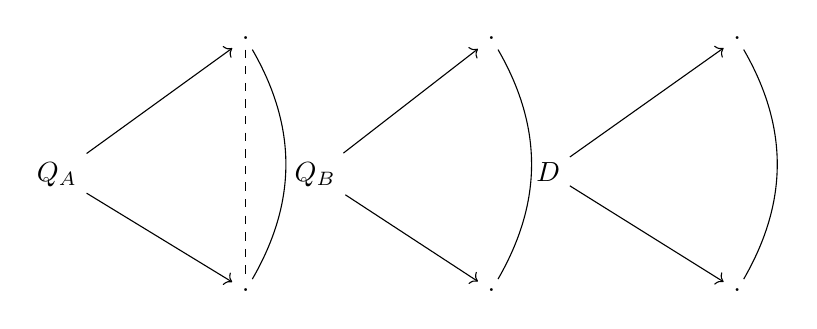
\begin{tikzpicture}[-, node distance = 3cm, scale=0.8]
        \node[anchor=north](HA){\(Q_A\)};
        \node[anchor=north](HA_d1) at (3, 2){.};
        \node[anchor=north](HA_d2) at (3, -2){.};
    
        \path[->] (HA) edge node {}(HA_d1);
        \path[->] (HA) edge node {}(HA_d2);
        \path (HA_d1) edge [bend left] node {}(HA_d2);
        \path (HA_d1) [dashed] edge node {}(HA_d2);
    
        \node[anchor=north](HB) at (4.1, 0){\(Q_B\)};
        \node[anchor=north](HB_d1) at (6.9, 2){.};
        \node[anchor=north](HB_d2) at (6.9, -2){.};
    
        \path[->] (HB) edge node {}(HB_d1);
        \path[->] (HB) edge node {}(HB_d2);
        \path(HB_d1) edge [bend left] node {}(HB_d2);
    
        \node[anchor=north](D) at (7.8, 0){\(D\)};
        \node[anchor=north](D_d1) at (10.8, 2){.};
        \node[anchor=north](D_d2) at (10.8, -2){.};
        
        \path[->] (D) edge node {}(D_d1);
        \path[->] (D) edge node {}(D_d2);
        \path(D_d1) edge [bend left] node {}(D_d2);
    \end{tikzpicture}
    \caption*{Figure 2 (revisited): Imperfect information Extensive Form Game 
    between the distributor and the 2 queueing systems}
\end{figure}

As described in section \ref{sec:model_overview} queueing system \(A\) decides
on a strategy, then queueing system \(B\) chooses its own threshold, unaware 
of the first queueing system's choice.
Finally, the distributor makes its choice based on the strategies that the 
queueing systems chose to play. 

The problem can be formulated by 3 matrices; the two payoff matrices of the 
normal form game and the routing matrix.
The payoff matrices and their utilities are defined by equations 
(\ref{eq:payoff-entry}) and (\ref{eq:payoff_matrices}) is section 
\ref{sec:model_overview}:

\begin{equation*}
    A = 
    \begin{pmatrix}
        U_{1,1}^A & U_{1,2}^A & \dots & U_{1,N_B}^A \\
        U_{2,1}^A & U_{2,2}^A & \dots & U_{2,N_B}^A \\
        \vdots & \vdots & \ddots & \vdots \\
        U_{N_A,1}^A & U_{N_A,2}^A & \dots & U_{N_A,N_B}^A \\
    \end{pmatrix},
    B = 
    \begin{pmatrix}
        U_{1,1}^B & U_{1,2}^B & \dots & U_{1,N_B}^B \\
        U_{2,1}^B & U_{2,2}^B & \dots & U_{2,N_B}^B \\
        \vdots & \vdots & \ddots & \vdots \\
        U_{N_A,1}^B & U_{N_A,2}^B & \dots & U_{N_A,N_B}^B \\
    \end{pmatrix}
    \tag{\ref{eq:payoff_matrices} revisited}
\end{equation*}


Similarly, the entries of the routing matrix are defined by equation 
(\ref{eq:obj_distributor}):
% TODO: Make sure this is defined PROPERLY and CONSISTENTLY in model_overview section or here in model_overview section or here
\begin{equation*}
    (p_A, p_B) \quad s.t. \quad 
    \alpha L_A(p_A) + (1 - \alpha) B_A(p_A) = 
    \alpha L_B(p_B) + (1 - \alpha) B_B(p_B)
    \tag{\ref{eq:obj_distributor} revisited}
\end{equation*}

Equation \ref{eq:obj_distributor} is properly defined and explained in section 
\ref{sec:model_overview}.
Thus, using equation \ref{eq:obj_distributor} for all possible sets of 
thresholds we can get the full routing matrix that consists of the proportions
to send to queueing system A (\(p_A\)) and to queueing system B (\(p_B\)).

\begin{equation}\label{eq:routing_matrix}
    R = 
    \begin{pmatrix}
        (p_{1,1}^A, p_{1,1}^B) & (p_{1,2}^A, p_{1,2}^B) & \dots & 
        (p_{1,N_B}^A, p_{1,N_B}^B) \\
        (p_{2,1}^A, p_{2,1}^B) & (p_{2,2}^A, p_{2,2}^B) & \dots & 
        (p_{2,N_B}^A, p_{2,N_B}^B) \\
        \vdots & \vdots & \ddots & \vdots \\
        (p_{N_A,1}^A, p_{N_A,1}^B) & (p_{N_A,2}^A, p_{N_A,2}^B) & \dots & 
        (p_{N_A,N_B}^A, p_{N_A,N_B}^B) \\
    \end{pmatrix}
\end{equation}

Note that since \(p_{i,j}^A + p_{i,j}^B = 1\) the routing matrix needs only to
store one of the two values; either \(p_{i,j}^A\) or \(p_{i,j}^B\).
Thus, the routing matrix \(R\) can be simplified to:

\begin{equation}\label{eq:routing_matrix_simplified}
    R = 
    \begin{pmatrix}
        p_{1,1}^A & p_{1,2}^A & \dots & p_{1,N_B}^A \\
        p_{2,1}^A & p_{2,2}^A & \dots & p_{2,N_B}^A \\
        \vdots & \vdots & \ddots & \vdots \\
        p_{N_A,1}^A & p_{N_A,2}^A & \dots & p_{N_A,N_B}^A \\
    \end{pmatrix}
\end{equation}

The game can thus be partitioned into a normal form game between the
two queueing systems and then finding the distributor's best strategy. 

\subsection{Backwards Induction}

In order to populate the payoff matrices and the routing matrix the method
of backwards induction is used.
Consider figure \ref{fig:imperfect-info-game} and the flow of the game that was
described (i.e. \(Q_A, Q_B \rightarrow D\)).
Due to the fact that the payoff matrices \(A\) and \(B\) depend on the routing 
matrix \(R\) the entries of the matrices are calculated in a backwards way 
(\(D \rightarrow Q_A, Q_B\)). 
Thus for every pair of strategies \(T_A, T_B\), the proportion of individuals 
that are to be transported to each queueing system is calculated first. 

Consider a game where the capacities of the two systems are \(N_A = 4\) and 
\(N_B = 3\).
The strategy space of players \(Q_A\) and \(Q_B\) would then be 
\(T_A = \{1, 2, 3, 4\}\) and \(T_B = \{1, 2, 3\}\) respectively.
Now, starting from an arbitrary starting point of \(T_A=1\) and \(T_B=1\), the
corresponding entry of the routing matrix the routing matrix can be calculated.
Using equation \ref{eq:obj_distributor} for \(T_A=1\) and \(T_B=1\):

\begin{equation*}
    (p_A, p_B) \quad s.t. \quad 
    \alpha L_A(p_A) + (1 - \alpha) B_A(p_A) = 
    \alpha L_B(p_B) + (1 - \alpha) B_B(p_B)
\end{equation*}

The above equation can be solved by using Brent's bisection algorithm.
% TODO: Cite Brent's algorithm
The calculated value of \(p_A\) corresponds to the entry on the first row and 
first column of the routing matrix:

\begin{equation}\label{eq:routing_matrix_1_1}
    R = 
    \begin{pmatrix}
        p_{1,1}^A & - & - \\
        - & - & - \\
        - & - & - \\
        - & - & - \\
    \end{pmatrix}
\end{equation}

In fact all remaining values of the routing matrix can be calculated by
solving \(N \times M\) similar equations using Brent's bisection algorithm.
Therefore, having calculated the entire routing matrix the payoff matrices can
be calculated.
Consider once again the case of \(T_A=1, T_B=1\). 

% TODO: Make sure this is defined PROPERLY and CONSISTENTLY in model_overview section or here
\begin{equation*}
    U_{1, 1}^A = \quad 1 -\left( 
        \hat{P} - P(W_A < R) 
    \right)^2,
    \quad
    U_{1, 1}^B = \quad 1 -\left( 
        \hat{P} - P(W_B < R) 
    \right)^2 \tag{\ref{eq:payoff-entry} revisited}
\end{equation*}

These are the utilities of players \(A\) and \(B\) when both players choose a
strategy of \(T = 1\).
% TODO: Change R everywhere to t
Here \(R\) is the predefined waiting time target to be met by a percentage of 
individuals \( \hat{P} \) and \(P(W_i < R)\) is properly defined in section
\ref{sec:proportion_within_target}.

\begin{equation}\label{eq:payoff_matrices_1_1}
    A = 
    \begin{pmatrix}
        U_{1, 1}^A & - & - \\
        - & - & - \\
        - & - & - \\
        - & - & - \\
    \end{pmatrix}, \quad
    B = 
    \begin{pmatrix}
        U_{1, 1}^B & - & - \\
        - & - & - \\
        - & - & - \\
        - & - & - \\
    \end{pmatrix}
\end{equation}

Similar to the routing matrix, the above procedure can be repeated for all 
possible values of \(T_A\) and \(T_B\) to populate all entries of the payoff 
matrices. 


\subsection{Nash Equilibrium}

\subsection{Learning Algorithms}

    \section{EMS - ED application}

\subsection{Application}

\subsection{Data Analysis}
    \section{Conclusion}

The motivation behind this study has been that emergency departments are 
under a lot of pressure to satisfy some regulations. 
This paper shows how this can negatively impact the pathway of both the 
ambulance patients and the ambulance service itself.
Due to some managerial decision making that takes place at the ED, ambulances 
stay blocked outside of the ED at the hospital's parking zone in an attempt
to satisfy these regulations.

This study explores a generic 3-player game theoretic model between the 
decision makers of two queueing systems and a service that distributes 
individuals to these two systems (section \ref{sec:model_overview}).
It also describes the construction of the underlying queueing theoretic model 
that has a tandem buffer and a single service centre (section 
\ref{sec:queueing_model}).
Furthermore, the formulas for the performance measures of the queueing model 
are also derived (sections \ref{sec:waiting_time}, \ref{sec:blocking_time}, 
\ref{sec:proportion_within_target}). 
This novel queuing model is the first contribution of the paper.
The game theoretic model is then applied to a healthcare scenario by looking at
the interface between the EDs and the EMS.
The inefficiencies that emerge from the perspective of the EMS were explored 
along with ways to apply some incentive mechanisms to improve them.
The key findings from this paper that were observed when playing the game
between two EDs and the EMS are:
\begin{itemize}
    \item Inefficiencies can be learned and emerge naturally
    \item Targeted incentivisation of behaviours can help escape inefficiencies
\end{itemize}
The former relates to the results of asymmetric replicator dynamics that showed 
that inefficient scenarios can arise by playing the game while the latter 
implies that the learned inefficiencies can be escaped by carefully applying 
certain incentives to the players.
This applied game theoretic model is the second main contribution of this paper.

The model presented here assumes the presence of two players that can receive 
individuals. 
However, in a realistic healthcare scenario an ambulance may have to decide 
among multiple EDs.
An immediate extension of this work would be to consider a multiplayer system
that could represent a group of hospitals in a concentrated area.
Additionally, the game theoretic model that was created uses a discrete 
strategy space for the EDs (something that is also present in various related 
literature~\cite{deo2011centralized, knight2017measuring}).
The single threshold parameter that is used for the ED's decision may not be 
the best way to describe the model.
In reality ED managers could have far more complex parameters for their 
decision making process.
Finally this work assumes that the EMS and EDs act in a selfish and rational
way by only aiming to satisfy their own objectives.
In fact, modelling behaviour in a healthcare setting is a much more complex 
task where some cooperation may often be observed.
Another extension would be to explore the behaviour of the ED staff via an 
agent-based model. 
This in turn can be used to model ED staff as agents each with their own 
behavioural traits.

    \newpage
    \bibliographystyle{plain}
    \bibliography{bibliography.bib}

    \begin{appendices}
    
    \section{Discrete Event Simulation}\label{sec:appendix_des}

% TODO: Include details of DES
    \section{Mean waiting time}\label{sec:appendix_mean_waiting}

    \section{Mean blocking time} \label{sec:appendix_mean_blocking}

The set of states where individuals can be blocked is defined as:
\begin{equation*}
    S_b = \{(u,v) \in S \; | \; u > 0\} 
    \tag{\ref{eq:set_of_blocking_states} revisited}
\end{equation*}

The mean sojourn time for each state is given by the inverse of the out-flow of
that state ~\cite{Stewart2019}.
However, whenever a type 2 individual arrives at the system, no subsequent 
arrival of another type 2 individual can affect its pathway or total time in 
the system.
Therefore, looking at the mean time in the system from the perspective of an 
individual of the second type, all such type 2 arrivals need to be ignored.
Note here that this is not the case for individuals of the first type.
Whenever a type 2 individual is blocked and a type 1 individual arrives the type
2 individuals will stay blocked for some additional amount of time.
Thus, the mean time that a type 2 individual spends at each state is given by:

\begin{equation*}
    c(u,v) = 
    \begin{cases}
        \frac{1}{\min(v,C) \mu}, & \text{if } v = N\\
        \frac{1}{\lambda_1 + \min(v,C) \mu}, & \text{otherwise}
    \end{cases} 
    \tag{\ref{eq:sojourn_blocking_time} revisited}
\end{equation*}

In equation (\ref{eq:sojourn_blocking_time}), both service completions and 
type 1 arrivals are considered. 
Thus, from a blocked individual's perspective whenever the system moves from one 
state \((u,v)\)
to another state it can either:

\begin{itemize}
    \item be because of a service being completed: we will denote the probability 
    of this happening by \(p_s(u,v)\). 
    \item be because of an arrival of an individual of type 1: denoting such 
    probability by \(p_a(u,v)\).
\end{itemize}
The probabilities are given by:

\begin{equation*}
    p_s(u,v) = \frac{\min(v,C)\mu}{\lambda_1 + \min(v,C)\mu}, \qquad
    p_a(u,v) = \frac{\lambda_1}{\lambda_1 + \min(v,C)\mu}
    \tag{\ref{eq:probs_of_service_and_arrival} revisited} 
\end{equation*}


Having defined \(c(u,v)\) and \(S_b\) a formula for the blocking time that is
expected to occur at each state can be given by:

    \begin{equation*}
    b(u,v) = 
    \begin{cases} 
        0, & \textbf{if } (u,v) \notin S_b \\
        c(u,v) + b(u - 1, v), & \textbf{if } v = N = T\\
        c(u,v) + b(u, v-1), & \textbf{if } v = N \neq T \\
        c(u,v) + p_s(u,v) b(u-1, v) + p_a(u,v) b(u, v+1), & \textbf{if } u > 0 
        \textbf{ and } \vspace{-0.2cm} \\ 
        & \quad v = T \\
        c(u,v) + p_s(u,v) b(u, v-1) + p_a(u,v) b(u, v+1), & \textbf{otherwise} \\
    \end{cases}
    \tag{\ref{eq:general_blocking_time_at_each_state} revisited}
\end{equation*}

A direct approach will be used to solve this equation here. 
By enumerating all equations of (\ref{eq:general_blocking_time_at_each_state}) 
for all states \((u,v)\) that belong in \(S_b\) 
a system of linear equations arises where the unknown variables are all the 
\(b(u,v)\) terms. 
Note here that these equations correspond to all blocking states as defined in
(\ref{eq:set_of_blocking_states}). 
Equations that correspond to non-blocking states have a value of \(0\) as 
defined in (\ref{eq:general_blocking_time_at_each_state})
The general form of the equation in terms of \(C,T,N \text{ and } M\) is given by: 

\begin{align}
    b(1,T) \quad &= \quad c(1, T) + p_a b(1, T + 1) \label{eq:first_eq_of_blocking_general}\\
    b(1,T + 1) \quad &= \quad c(1, T + 1) + p_s b(1, T) + p_a b(1, T + 1) \\
    b(1,T + 2) \quad &= \quad c(1, T + 2) + p_s b(1, T + 1) + p_a b(1, T + 3) \\
    & \ \, \vdots \nonumber \\
    b(1, N) \quad &= \quad c(1, N) + b(1, N - 1) \\
    b(2, T) \quad &= \quad c(2, T) + p_s b(1, T) + p_a b(2, T + 1) \\
    b(2, T + 1) \quad &= \quad c(2, T + 1) + p_s b(2, T) + p_a b(2, T + 2) \\
    & \ \, \vdots \nonumber \\
    b(M - 1, N) \quad &= \quad c(M, N - 1) + b(M, N-1) \\ 
    b(M, T) \quad &= \quad c(T, N) + p_s b(T-1, N) + p_a b(T, N+1) \\
    & \ \, \vdots \nonumber \\
    b(M, N) \quad &= \quad c(M, N) + b(M, N-1) \label{eq:last_eq_of_blocking_general}
\end{align}

The equivalent matrix notation of the linear system of equations 
(\ref{eq:first_eq_of_blocking_general}) - (\ref{eq:last_eq_of_blocking_general})
is given by \(Zx=y\), where:
\begin{equation}
    \scalebox{0.73}{\(
        Z = 
        \begin{pmatrix}
            -1 & p_a & 0 & \dots & 0 & 0 & 0 & 0 & 0 & \dots & 0 & 0 \\ %(1,T)
            p_s & -1 & p_a & \dots & 0 & 0 & 0 & 0 & 0 & \dots & 0 & 0 \\ %(1,T+1)
            0 & p_s & -1 & \dots & 0 & 0 & 0 & 0 & 0 & \dots & 0 & 0 \\ %(1,T+2)
            \vdots & \vdots & \vdots & \ddots & \vdots & \vdots & \vdots & 
            \vdots & \vdots & \ddots & \vdots & \vdots \\ 
            0 & 0 & 0 & \dots & 1 & -1 & 0 & 0 & 0 & \dots & 0 & 0 \\ %(1,N)
            p_s & 0 & 0 & \dots & 0 & 0 & -1 & p_a & 0 & \dots & 0 & 0 \\ %(2,T)
            0 & 0 & 0 & \dots & 0 & 0 & p_s & -1 & p_a & \dots & 0 & 0 \\ %(2,T+1)
            \vdots & \vdots & \vdots & \ddots & \vdots & \vdots & \vdots & 
            \vdots & \vdots & \ddots & \vdots & \vdots \\ 
            0 & 0 & 0 & \dots & 0 & 0 & 0 & 0 & 0 & \dots & 1 & -1 \\ %(M,N)
        \end{pmatrix},
        x = 
        \begin{pmatrix}
            b(1,T) \\
            b(1,T+1) \\
            b(1,T+2) \\
            \vdots \\
            b(1,N) \\
            b(2,T) \\
            b(2,T+1) \\
            \vdots \\
            b(M,N) \\
        \end{pmatrix}, 
        y= 
        \begin{pmatrix}
            -c(1,T) \\
            -c(1,T+1) \\
            -c(1,T+2) \\
            \vdots \\
            -c(1,N) \\
            -c(2,T) \\
            -c(2,T+1) \\
            \vdots \\
            -c(M,N) \\
        \end{pmatrix}
    \)} \tag{\ref{eq:general_algebaric_approach_blocking_time} revisited}
    \end{equation}

    The elements of the matrix \(Z\) can be acquired using \(Z_{ij}\) defined in 
    equation (\ref{eq:general_mapping_function_of_blocking_matrix}) where \(i\) 
    and \(j\) are states \((u_i, v_i), (u_j, v_j) \in S_b\) 
    (\ref{eq:set_of_blocking_states}).

    \begin{equation}
    Z_{ij} = 
    \begin{cases}
        p_a, & \textbf{if } j = i + 1 \textbf{ and } v_i \neq N \\
        p_s, & \textbf{if } j = i - 1 \textbf{ and } v_i \neq N, v_i \neq T \\
            & \textbf{or } j = i - N + T \textbf{ and } u_i \geq 2,\,v_i = T \\
        1, & \textbf{if } j = i - 1 \textbf{ and } v_i = N \\
        -1, & \textbf{if } i = j \\
        0, & \textbf{otherwise} \\
    \end{cases}
    \tag{\ref{eq:general_mapping_function_of_blocking_matrix} revisited}
\end{equation}


Thus, having calculated the mean blocking time for all blocking states 
\(b(u,v)\), they can be combined together in a formula.
The resultant formula for the mean blocking time is given by:

\begin{equation}
    B = \frac{\sum_{(u,v) \in S_A} \pi_{(u,v)} \; b(u,v)}{\sum_{(u,v) \in S_A} 
    \pi_{(u,v)}} \tag{\ref{eq:algebraic_blocking_time} revisited}
\end{equation}

To illustrate how the described formula works consider a Markov model where 
\(C=2, T=2, N=4, M=2\) (figure \ref{fig:example_algeb_blocking}). 
The equations that correspond to such a model are shown in 
(\ref{eq:first_eq_of_blocking_example})-(\ref{eq:last_eq_of_blocking_example}) 
and their equivalent matrix notation form is shown in 
(\ref{eq:example_algebaric_approach_blocking_time}).

\begin{minipage}{.5\textwidth}
    \begin{figure}[H]
        \scalebox{0.6}{\documentclass{article}

\usepackage{amsmath}
\usepackage{amsfonts} 
\usepackage{geometry}
\usepackage{multicol}
\usepackage{float}
% \usepackage{mathtools}
% \usepackage{graphicx}
% \usepackage{soul}
% \usepackage{indentfirst}
\usepackage{tikz}
\usetikzlibrary{calc, automata, chains, arrows.meta, math}
\setcounter{MaxMatrixCols}{20}


\title{A game theoretic model of the behavioural gaming that takes place at the EMS - ED interface}

\author{
    Michalis Panayides, 
    Paul Harper, 
    Vince Knight
}

\begin{document}

\maketitle

\input{Abstract/main.tex}


\newpage
\tableofcontents

\newpage
\input{Introduction/main.tex}

\newpage
\input{Game_theory_component/main.tex}

\newpage
\input{MarkovChain/markov_chain_model/main.tex}
\input{MarkovChain/expressions_from_pi/main.tex}
\input{MarkovChain/markov_example/main.tex}

\newpage
\input{BehaviouralMethodology/main.tex}

\newpage
\input{Application_EMS_ED/main.tex}

\newpage
\input{Conclusion/main.tex}


\end{document}}
        \caption{
            \centering{Example of Markov chain with \(C=2, T=2, N=4, M=2\)}
        }
        \label{fig:example_algeb_blocking}
    \end{figure}
    \end{minipage}
    \begin{minipage}{.43\textwidth}
    \begin{align}
        b(1,2) &= c(1,2) + p_a b(1,3) \label{eq:first_eq_of_blocking_example} \\
        b(1,3) &= c(1,3) + p_s b(1,2) \nonumber \\ &+ p_a b(1,4) \\
        b(1,4) &= c(1,4) + b(1,3) \\
        b(2,2) &= c(2,2) + p_s b(1,2) \nonumber \\ &+ p_a b(2,3) \\
        b(2,3) &= c(2,3) + p_s b(2,2) \nonumber \\ &+ p_a b(1,4) \\
        b(2,4) &= c(2,4) + b(2,3) \label{eq:last_eq_of_blocking_example}
    \end{align}
\end{minipage}

\begin{equation}\label{eq:example_algebaric_approach_blocking_time}
    Z=
    \begin{pmatrix}
        -1 & p_a & 0 & 0 & 0 & 0 \\ %(1,2)
        p_s & -1 & p_a & 0 & 0 & 0 \\ %(1,3)
        0 & 1 & -1 & 0 & 0 & 0 \\ %(1,4)
        p_s & 0 & 0 & -1 & p_a & 0\\ %(2,2)
        0 & 0 & 0 & p_s & -1 & p_a \\ %(2,3)
        0 & 0 & 0 & 0 & 1 & -1 \\ %(2,4)
    \end{pmatrix},
    x=
    \begin{pmatrix}
        b(1,2) \\
        b(1,3) \\
        b(1,4) \\
        b(2,2) \\
        b(2,3) \\
        b(2,4) \\
    \end{pmatrix}, 
    y=
    \begin{pmatrix}
        -c(1,2) \\
        -c(1,3) \\
        -c(1,4) \\
        -c(2,2) \\
        -c(2,3) \\
        -c(2,4) \\
    \end{pmatrix}
\end{equation}

    \section{Mean blocking time} \label{sec:appendix_mean_proportion}
    
    \section{Type 1 and type 2 performance measure comparisons using simulation and
Markov chains}\label{sec:appendix_additional_figures}

\begin{figure}[H]
    \centering
    \includegraphics[width=.7\textwidth]{imgs/waiting_time_comparison/waiting_1.pdf}
    \caption{
        Comparison of mean waiting time for type 1 individuals between values 
        obtained from the Markov chain formulas and values obtained from 
        simulation.
    }
    \label{fig:markov_vs_des_waiting_time_comparison_1}
\end{figure}

\begin{figure}[H]
    \centering
    \includegraphics[width=.7\textwidth]{imgs/waiting_time_comparison/waiting_2.pdf}
    \caption{
        Comparison of mean waiting time for type 2 individuals between values 
        obtained from the Markov chain formulas and values obtained from 
        simulation.
    }
    \label{fig:markov_vs_des_waiting_time_comparison_2}
\end{figure}

\begin{figure}[H]
    \centering
    \includegraphics[width=.7\textwidth]{imgs/proportion_within_target_comparison/proportion_1.pdf}
    \caption{
        Comparison of proportion within target time for type 1 individuals 
        between values obtained from the Markov chain formulas and values 
        obtained from simulation. 
    }
    \label{fig:markov_vs_des_proportion_comparison_1}
\end{figure}

\begin{figure}[H]
    \centering
    \includegraphics[width=.7\textwidth]{imgs/proportion_within_target_comparison/proportion_2.pdf}
    \caption{
        Comparison of proportion within target time for type 2 individuals 
        between values obtained from the Markov chain formulas and values 
        obtained from simulation. 
    }
    \label{fig:markov_vs_des_proportion_comparison_2}
\end{figure}
    
\end{appendices}
      
\end{document}